\documentclass{amsbook}
\usepackage[english]{babel}
\usepackage{graphicx}
\usepackage[pdfborder={0,0,0},colorlinks=true,linkcolor=blue,urlcolor=red]{hyperref}
\begin{document}
\title{ECO32 User Manual}
\author{Martin Geisse}
\maketitle

\newcommand{\mylabel}[1]{\label{#1}}
\newcommand{\myref}[2]{\hyperref[#2]{Chapter #1, Section \ref{#2}}}

\newcommand{\definition}[1]{{\it #1}}
\newcommand{\name}[1]{{\it #1}}

\newcommand{\eco}{{\sc ECO32} }
\newcommand{\ecox}{{\sc ECO32}}
\newcommand{\pc}{{\sc PC} }
\newcommand{\pcx}{{\sc PC}}
\newcommand{\psw}{{\sc PSW} }
\newcommand{\pswx}{{\sc PSW}}
\newcommand{\mmu}{{\sc MMU} }
\newcommand{\mmux}{{\sc MMU}}

\tableofcontents
\chapter{Introduction}
The ECO32 is a general-purpose 32-bit RISC soft-core microprocessor, to be
implemented on an FPGA. It was originally designed to understand the RISC
architecture as described by Hennessy and Patterson in their books. The
current version is a simple, albeit slow implementation of the instruction
set architecture described in this manual. Future versions will include
various optimizations to make the ECO32 feasible for real-world projects.

\section{Features}
The \eco supports the following features:
\begin{itemize}
\item Soft-core processor to be implemented on an FPGA
\item 32 general-purpose registers, each 32 bits wide
\item 32-bit ALU, shifter, multiplication and division units
\item load/store architecture
\item 32-bit unified instruction and data address space
\item 16 external interrupt lines
\item two privilege modes to execute both trusted and untrusted code
\item paged virtual memory with a page size of 4K
\item assembler, instruction-set simulator, and C compiler support
\end{itemize}

\section{Requirements}
So far, the \eco has only been implemented on a Xilinx Spartan-3 FPGA. Implementing it on other FPGAs may cause problems if the \eco uses device primitives that are not supported on the target platform.

\chapter{ECO32 Architecture}
\mylabel{architecture}

The \eco is a general-purpose 32-bit RISC processor. Its instruction set is tailored to handle only the most basic computation steps at once, and to allow arbitrary combination of these basic steps for full flexibility. Instructions are executed sequentially. The \eco also includes the basic mechanisms to implement modern operating systems, such as interrupts, privileged instructions, and virtual memory. Operations on floating-point data types are not supported.

The \eco is a soft-core that must be used in a larger system-on-chip (SoC) design inside a field programmable gate array (FPGA). The \eco is connected to other on-chip resources using a uniform SoC bus architecture. These resources include a RAM controller, a ROM controller, and peripheral devices such as coprocessors, communication controllers, and controllers for external devices.

\section{Data Types}
\mylabel{data_types}

The following basic data types are processed by the \eco:
\begin{itemize}
\item \definition{Byte}: A unit of 8 bits
\item \definition{Half-Word}: A unit of 16 bits
\item \definition{Word}: A unit of 32 bits
\end{itemize}
The bits of each unit are written down starting from the most-significant bit to the least significant bit.

The size of the basic units allows the arrangement of bytes as half-words, or of bytes or half-words as words. Two common kinds of arrangements are defined for sequences of bytes or half-words. Let $a = (a_7, ..., a_0)$, $b = (b_7, ..., b_0)$, $c = (c_7, ..., c_0)$, and $d = (d_7, ..., d_0)$ be byte values, and $p = (p_{15}, ..., p_0)$ and $q = (q_{15}, ..., q_0)$ be half-word values. 
\begin{itemize}
\item \definition{Big Endian} arrangement maps
\begin{itemize}
\item the byte sequence $(a, b)$ to the half-word $(a_7, ..., a_0, b_7, ..., b_0)$,
\item the byte sequence $(a, b, c, d)$ to the word\\$(a_7, ..., a_0, b_7, ..., b_0, c_7, ..., c_0, d_7, ..., d_0)$, and
\item the half-word sequence $(p, q)$ to the word $(p_{15}, ..., p_0, q_{15}, ..., q_0)$.
\end{itemize}
\item \definition{Little Endian} arrangement maps
\begin{itemize}
\item the byte sequence $(a, b)$ to the half-word $(b_7, ..., b_0, a_7, ..., a_0)$, 
\item the byte sequence $(a, b, c, d)$ to the word\\$(d_7, ..., d_0, c_7, ..., c_0, b_7, ..., b_0, a_7, ..., a_0)$, and
\item the half-word sequence $(p, q)$ to the word $(q_{15}, ..., q_0, p_{15}, ..., p_0)$.
\end{itemize}
\end{itemize}

When units of several bits are interpreted as numbers, two different schemes are used. An \definition{unsigned} interpretation maps the bits $(a_N, ..., a_0)$ to the number $\sum_{i=0}^N a_i2^i$. A \definition{signed} (or \definition{two's complement}) interpretation maps the same bit sequence to the number $-a_N2^N + \sum_{i=0}^{N-1}a_i2^i$.

The functions $signed$ and $unsigned$ shall denote signed and unsigned interpretation of a bit sequence as a number, respectively.

A bit sequence $(a_N, ..., a_0)$ is \definition{truncated} to $M \leq N$ bits by taking the bit sequence $(a_M, ..., a_0)$. The same bit sequence is \definition{zero-extended} to $P \geq N$ bits by taking $(0, ..., 0, a_N, ..., a_0)$, or \definition{sign-extended} to $P$ bits by taking $(a_N, ..., a_N, a_{N-1}, ..., a_0)$. Zero-extension and sign-extension preserve the unsigned or signed interpretation, respectively, if the value can be represented in the target number of bits at all.

The function $truncate_N$ shall denote truncation to $N$ bits, $zeroext_N$ shall denote zero-extension to $N$ bits, and $signext_N$ shall denote sign-extension to N bits.

\section{Addresses}
\mylabel{addresses}

An \definition{address} is a 32-bit unsigned value that indicates a location in RAM, ROM, or in a peripheral device. An address is \definition{half-word-aligned} if it is divisible by 2, that is, its least significant bit is 0. An address is \definition{word-aligned} if it is divisible by 4, that is, its two least significant bits are 0. The design of the \eco ensures that all accesses to the RAM, ROM, or to peripheral devices are aligned with respect to the transferred data size.

The \eco distinguishes \name{virtual} and \name{physical} addresses. Virtual addresses are generated by a program to address RAM or device locations. Virtual addresses are converted to physical addresses by the memory management unit. Finally, physical addresses select locations in RAM, ROM, or peripheral devices. See \myref{2}{mmu} for details.

The mapping is always defined in such a way that a virtual address is half-word (word) aligned if and only if the corresponding physical address is. Any attempt to access a half-word (word) sized location at an address that is not half-word (word) aligned is called a \definition{misaligned} access and triggers a fault.

Each physical address in the range 0x00000000 through 0x2FFFFFFF selects a byte-sized location in RAM or ROM. Each half-word (word) aligned address in that range selects a half-word (word) in RAM or ROM comprising the corresponding byte locations in a big-endian fashion.

Each word-aligned physical address in the range 0x30000000 through 0x3FFFFFFF selects a word-sized location in a peripheral device. Byte or half-word sized access to peripheral devices is not allowed and the effect of such accesses on the device and on values read is undefined.

Physical addresses in the range 0x40000000 through 0xFFFFFFFF are not used.

\section{Program Counter (PC)}
\mylabel{pc}

The \pc is a 32-bit virtual address register that contains the address of the next instruction to execute. Each instruction is 32 bits, or 4 bytes wide. An instruction is \definition{fetched} by loading a word value from the virtual address given by the \pcx, then incrementing it by 4 (thus moving to the next instruction). If the execution of the instruction later modifies the \pcx, it is this new value that is modified.

\section{General-Purpose Registers}
\mylabel{general_purpose_registers}

Most data processing occurs in a set of 32 general-purpose registers, each 32 bits wide. Instructions exist to perform arithmetic operations, logic operations, multiplication and division, and data type conversion. Such operations load the operands from general-purpose registers, perform the computation, and store the result back in a general-purpose register. General-purpose registers also hold the addresses and data for transfers to and from RAM, ROM, and peripheral devices. The interpretation of a value in a general-purpose register as data or address depends solely on the instructions that operate on that value -- the value itself is an untyped 32-bit unit.

Some general-purpose registers have a special function in addition to their
regular behaviour:
\begin{itemize}
\item Register \#0 is not actually backed by a physical register. Reading from
this register always yields the value 0. Writing to this register has no
effect. Register \#0 can be exploited in various cases where a value of zero is
needed in a register, without first loading that value into a register.
\item Registers \#1 through \#29 do not serve any special purpose.
\item Register \#30 is used to store the return address when an exception occurs.
That value is later used by the exception service routine to return to the
place where the exception had occurred. At any time when interrupts are
enabled, this register may not be used, because its value could be overwritten
by an unexpected interrupt.
\item Register \#31 is used to store the return address in a subroutine call.
\end{itemize}

\section{Load/Store Architecture}
\mylabel{load_store_architecture}

Specific instructions exist to transfer data to or from RAM, ROM, or peripheral devices. No such data transfer occurs except for these instructions, as well as instruction fetching itself. That is, all other instructions operate entirely inside the \eco.

A \definition{load} instruction transfers data from an external source into a general-purpose register. A \definition{store} instruction transfers data from a general-purpose register to an external target. The virtual address of the external source or target is determined by taking the value of a general-purpose register and adding a constant value that is encoded into the instruction.

Load and store instructions come in variants of word, half-word, and byte transfers with respect to the size of the transferred data. The address computation is not affected by the transfer size, but the resulting address must be aligned to the transfer size. A word transfer affects a full 32-bit general purpose register. A half-word or byte store instruction transfers only the lower 16 or 8 bits, respectively. An unsigned half-word load instruction loads 16 bits from an external source, zero-extends it to 32 bits, and stores the result in a general-purpose register. Similarly, a signed half-word load instruction sign-extends the value to 32 bits. Byte-sized load instructions work analogously.

\section{Special-Purpose Registers}
\mylabel{special_purpose_registers}

The \eco contains a set of special-purpose registers that are not used for computation, address generation, or data transfer. Instead, these registers control operation of the processor itself. Special purpose registers are accessed with the MVFS and MVTS instructions.

The following special-purpose registers are present in the \ecox:

\begin{tabular}{|c|c|}
\hline
Index & Name\\
\hline
0 & PSW\\
\hline
1 & TLB Index\\
\hline
2 & TLB Entry High\\
\hline
3 & TLB Entry Low\\
\hline
4 & TLB Bad Address\\
\hline
\end{tabular}

The first special register is the processor status word (\pswx). This register contains the main control parameters for the processor. See \myref{2}{psw} for details. The \psw can only be accessed from Kernel Mode.

The remaining special-purpose registers are used to communicate with the memory management unit. See \myref{2}{mmu} for details. The \mmu registers can only be accessed from Kernel Mode.

\section{Processor Status Word (PSW)}
\mylabel{psw}

The \psw controls execution in various way. It is actually a collection of fields, each of which has its own purpose and effect:

\begin{tabular}{|c|c|l|}
\hline
Bit Index & Name & Meaning\\
\hline
31..28 & --- & (ignored) \\
27 & $V$ & Exception Service Routine Vector. \\
26 & $U_C$ & Current privilege mode.\\
25 & $U_P$ & Previous privilege mode.\\
24 & $U_O$ & Old privilege mode.\\
23 & $I_C$ & Current global interrupt enable.\\
22 & $I_P$ & Previous global interrupt enable.\\
21 & $I_O$ & Old global interrupt enable.\\
20..16 & $EID$ & Exception identifier.\\
15..0 & $IEN$ & Channel-specific interrupt enable.\\
\hline
\end{tabular}

\subsection{Exception Service Routine Vector}
\mylabel{v_bit}

The $V$ bit of the \psw specifies the address of the exception service routines. If the V bit is 0, then service routines are located at a high physical address that lies at the beginning of the ROM. If the V bit is 1, then service routines are located at a low physical address that lies at the beginning of the RAM. See \myref{2}{service_routine_address} for details.

\subsection{Privilege Modes}
\mylabel{privilege_modes}

The $U_C$, $U_P$, and $U_O$ bits of the \psw form a three-level stack, with $U_C$ at the top. A bit value $X$ is \definition{pushed on} that stack by the following sequence:
\begin{itemize}
\item[] $U_O \leftarrow U_P$
\item[] $U_P \leftarrow U_C$
\item[] $U_C \leftarrow X$
\end{itemize}
A value is \definition{popped off} the stack by the following sequence:
\begin{itemize}
\item[] $U_C \leftarrow U_P$
\item[] $U_P \leftarrow U_O$
\end{itemize}

Only $U_C$ affects execution directly. If $U_C$ is 0, then the \eco runs in \definition{Kernel Mode} and can access privileged instructions and privileged addresses. If $U_C$ is 1, then the \eco runs in \definition{User Mode}, and any attempt to access a privileged instruction or privileged address will result in a \name{Privileged Instruction Fault} or \name{Privileged Address Fault}, respectively. When any exception is accepted, a value of 0 is pushed onto the three-level stack to enter \name{Kernel Mode}, and $U_O$ is discarded. The RFX instruction pops the topmost value off the stack to restore the execution state before the exception.

A privileged address is any virtual address in the range 0x80000000 through 0xFFFFFFFF. This range is reserved for the operating system, and includes both a page-mapped range from 0x80000000 through 0xBFFFFFFF, and a direct-mapped range from 0xC0000000 through 0xFFFFFFFF. See \myref{2}{mmu} for details.

\subsection{Interrupt Enable}
\mylabel{ien}

The $I_C$, $I_P$, and $I_O$ bits of the \psw form a three-level stack, with $I_C$ at the top. A bit value $X$ is \definition{pushed on} that stack by the following sequence:
\begin{itemize}
\item[] $I_O \leftarrow I_P$
\item[] $I_P \leftarrow I_C$
\item[] $I_C \leftarrow X$
\end{itemize}
A value is \definition{popped off} the stack by the following sequence:
\begin{itemize}
\item[] $I_C \leftarrow I_P$
\item[] $I_P \leftarrow I_O$
\end{itemize}

Only $I_C$ affects execution directly. If $I_C$ is 0, then interrupts are globally disabled. If any device signals an interrupt while $I_C$ is 0, then admission of that interrupt is postponed. If $I_C$ is 1, then interrupts are globally enabled (note that interrupts may still be disabled on a per-channel basis, see below). When any exception is accepted, a value of 0 is pushed onto the three-level stack to disable all interrupts, and $I_O$ is discarded. The RFX instruction pops the topmost value off the stack to restore the execution state before the exception.

The $IEN$ field controls admission of interrupts on a per-channel basis. An interrupt is only  accepted if both the global $I_C$ and the corresponding bit of the $IEN$ are set. Otherwise, admission of the interrupt is postponed until this condition arises. An interrupt may be {\it overlooked} if the device negates the interrupt signal again before $I_C$ and the corresponding $IEN$ bit are both set.

\subsection{Exception Identifier}
\mylabel{eid}

When an exception is accepted, the $EID$ field of the \psw is loaded with a number that identifies the cause of the exception. The meaning of these numbers is defined in the following table:

\begin{tabular}{|l|l|}
\hline
Value & Meaning \\
\hline
0..15 & Device Interrupt 0..15\\
16 & Bus Timeout\\
17 & Illegal Instruction\\
18 & Privileged Instruction\\
19 & Division by Zero\\
20 & Trap Instruction\\
21 & TLB Miss\\
22 & TLB Write\\
23 & TLB Invalid\\
24 & Illegal Address\\
25 & Privileged Address\\
26..31 & (unused - never loaded by the hardware)\\
\hline
\end{tabular}

\section{Exceptions: Interrupts and Faults}
\mylabel{exceptions}

An \definition{Exception} is a control transfer from user code to operating system code. There are two kinds of exceptions: An \definition{Interrupt} occurs when a peripheral device needs the attention of the \ecox. A \definition{Fault} occurs when the execution of an instruction fails.

Interrupts are only accepted between the execution of two instructions, and only if the $I_C$ and $IEN$ fields of the \psw allow so (see \myref{2}{ien}). Operating system code can control these fields to disable interrupts during time-critical code sequences or to achieve mutual exclusion. Typically, the interrupt service routine communicates with the device that caused the interrupt, then returns to the interrupted code and continues its execution as if nothing had happened (except that register \#30 had been overwritten, see below). Register \#30 should not be used for computations, since it would lose its value during an unexpected interrupt.

Faults occur during the execution of an instruction. Typically, a fault service routine would either correct the problem and restart the failed instruction, or terminate the corresponding program. In certain cases, a fault indicates a voluntary control transfer to the operating system to perform some action on behalf of the user program. In that case, the fault service routine would not restart the faulting instruction, but return to the instruction immediately following it.

\subsection{Accepting an Exception}
\mylabel{accept_exception}

When an exception is accepted, the following steps are taken automatically by the \eco:
\begin{enumerate}
\item Store the return address in the general-purpose register \#30. For interrupts (which occur between two instructions), this is the address of the instruction directly following the occurence of the interrupt. For faults, this is the address of the faulting instruction. Note that although fetching the faulting instruction had already increased
the PC by 4, a fault subtracts 4 again to obtain the original address of that instruction.
\item Push 0 on the $(I_C, I_P, I_O)$ stack in the \psw to disable interrupts, and to remember the previous interrupt enable state.
\item Push 0 on the $(U_C, U_P, U_O)$ stack in the \psw to enter Kernel Mode, and to remember the previous privilege mode.
\item Set the $EID$ field of the \psw to the corresponding exception identifier (see \myref{2}{eid})
\item Load the address of the service routine into the PC register (see \myref{2}{service_routine_address})
\end{enumerate}

\subsection{Exception Service Routine Addresses}
\mylabel{service_routine_address}

The address of the exception service routine, that is, the value loaded into the \pcx, is determined as follows. First, a base address is computed depending on the value of the $V$ field of the \pswx. If the $V$ bit is 0, then the base address is E0000000. If the $V$ bit is 1, then the base address is C0000000. Since these addresses are loaded into the \pcx, they are virtual. With $V$ set to 0, the address is a direct-mapped address that denotes the physical address 0x20000000, i.e. the first address associated with the ROM. With $V$ set to 1, the address is a direct-mapped address that denotes the physical address 0x00000000, i.e. the first address associated with the RAM. The $V$ bit can therefore be used to handle exceptions in a service routine located in ROM directly after startup, as well as handle them in a service routine located in RAM once an operating system is loaded.

Next, the cause of the exception is inspected. One specific kind of fault, the User Space TLB Miss, is given special treatment. For this fault, the actual address of the service routine is (base address + 8). For all other faults, as well as for all interrupts, the address of the service routine is (base address + 4). This leaves only enough space for a single instruction at (base address + 4), which is therefore typically a jump instruction. The special treatment for User Space TLB misses allows very fast handling of such faults. 

\subsection{Returning Control}
\mylabel{rfx}

The exception service routine of the operating system can then handle the exception. When the service routine is finished, it typically returns control:
\begin{itemize}
\item An interrupt service routine would return to the saved address in register \#30 to continue the interrupted code.
\item A fault service routine that has corrected a problem with the faulting instruction would reutrn to the saved address in register \#30 to restart that instruction.
\item A fault service routine that could not correct the problem would not return control. What happens in that case depends on the operating system architecture.
\item A fault service routine that performs an action on behalf of a user code request would not return to the faulting instruction, but to the instruction immediately following it. This can be achieved by adding 4 to register \#30 before returning.
\end{itemize}

A single instruction called RFX (return from exception) handles all these cases. This instruction performs the following sequence:
\begin{enumerate}
\item Load the value in register \#30 into the PC.
\item Restore the remembered state of the interrupt enable flag and privilege mode by popping the top value off the $(I_C, I_P, I_O)$ and $(U_C, U_P, U_O)$ stacks.
\end{enumerate}

\section{Memory Management Unit (MMU)}
\mylabel{mmu}

All addresses generated by the \ecox, including both the \pc as well as those from load and store instructions, are \definition{virtual} addresses. These addresses are transformed to \definition{physical} addresses by the memory management unit (MMU). The physical addresses are finally sent over the SoC bus to the memory controller or to peripheral hardware.

The memory management unit (MMU) distinguishes two parts of the virtual address space and uses different mapping algorithms for them. The page-mapped space ranges from virtual address 0x00000000 through 0xBFFFFFFF. The direct-mapped space ranges from virtual address 0xC0000000 through 0xFFFFFFFF. Note that this leaves the direct-mapped space entirely in the range of privileged addresses, such that only operating system code can access direct-mapped addresses.

\subsection{Direct-Mapped Space}

Virtual addresses in the direct-mapped space are transformed to physical addresses by subtracting the start address of that space, 0xC0000000. Thus, the direct-mapped space can be used to directly access any RAM, ROM, or device location in the physical address space.

\subsection{Page-Mapped Space}

Virtual addresses in the page-mapped space are subdivided into blocks of 4096 bytes called \definition{pages}. Each page is a continuous range of 4096 virtual addresses, and is mapped to a continuous range of 4096 physical addresses called a \definition{page frame}. Both pages and page frames are aligned to their size. Thus, in the page-mapped space, the upper 20 bits of the physical address (the \definition{page frame number}) are computed through a mapping function from the upper 20 bits of the virtual address (the \definition{page number}), and the 12 lower bits of the physical address are directly taken from the 12 lower bits of the virtual address.

The mapping function from pages to page frames can be defined and implemented freely by the operating system. No overall representation of the mapping is implemented by the \eco itself. Specifically, the \eco does not have a notion of a \name{page table} as found in other architectures. Instead, the mapping of pages to page frames is defined by a software function implemented by the operating system, and the results of that function are cached in a special memory called the \definition{translation look-aside buffer} (\definition{TLB}).

\subsection{Translation Lookaside Buffer (TLB)}

The TLB is a table of 32 entries, each mapping a 20-bit page number to a 20-bit page frame number. Both numbers are stored in an entry. When accessing a page-mapped virtual address, the TLB is searched for the page number. If an entry is found, then its page frame number is concatenated with the 12-bit page local address to yield the physical address. It is an error to have two entries with the same virtual page number, and the result of the mapping is undefined in that case. Having two entries with the same physical page number is fine however, and can be used to {\it mirror} a physical page frame at multiple virtual pages.

A full page mapping function is defined by $(2^{20} - 2^{18})$ mappings of pages to page frames. The 32 TLB entries contain a subset of these mappings, preferably those that are most needed in the near future. By writing to the TLB, a different subset can be loaded. It is also possible to change the mapping function itself by removing (overwriting) the old TLB entries and filling in the mappings of the new function.  The \eco is not concerned with the notion of the overall mapping function, but simply searches the TLB for a matching page number.

Each TLB entry always contains a mapping from a virtual page to a physical page frame. However, entries can be effectively {\it blanked} by entering a never-occuring page number. For example, virtual addresses in the range 0xC0000000 through 0xFFFFFFFF are direct-mapped, and thus never occur as virtual addresses in a TLB lookup.

In no entry is found in a lookup, a \name{TLB Miss Fault} occurs. This is either a \name{User Space TLB Miss} if the virtual address is in the range 0x00000000 through 0x7FFFFFFF (that is, it is an unprivileged address), or a \name{Kernel Space TLB Miss} if the virtual address is in the range 0x80000000 through 0xBFFFFFFF (that is, it is a privileged address). The control transfer to the service routine works slightly different for privileged and unprivileged addresses (see \myref{2}{service_routine_address}). The service routine for \name{TLB Miss Faults} typically loads an appropriate mapping into the TLB, then executes the RFX instruction to restart the failed instruction. In terms of an overall mapping function, the TLB miss service routine moves the TLB to a different subset of the mapping function, such that the new subset contains the faulting address.

\subsection{TLB Entry Flags}

TLB entries may be flagged {\it valid} (the {\it valid} flag is set) or {\it invalid} (the {\it valid} flag is not set), and they may be flagged {\it writeable} (the {\it write} flag is set) or {\it write-protected} (the {\it write} flag is not set). These flags only come to effect in a TLB entry whose page number is found during a lookup. If the valid flag is not set for such an entry, then a \name{TLB Invalid Fault} is triggered. If the write flag is not set for such an entry and the access is a write access, then a \name{TLB Write Fault} is triggered. Otherwise, the access succeeds. 

Note that the name of the {\it valid} flag is slightly misleading. The name might suggest that unsetting this flag marks a TLB entry as invalid and causes the lookup algorithm to overlook that entry. However, unsetting the {\it valid} flag actually marks the corresponding {\it page} as invalid and does not interfere with the lookup algorithm; instead, when the entry is found during lookup, it triggers a \name{TLB Invalid Fault}. To mark a TLB entry invalid and thus cause the lookup algorithm to overlook that entry, place an unused virtual page number into the entry, such as a page number from the direct-mapped virtual address range (0xC0000000 through 0xFFFFFFFF).

\subsection{Random Replacement and Fixed TLB Entries}
\mylabel{tlb_random}

The TLB miss service routine typically replaces a TLB entry with a mapping for the faulting address, then restarts the faulting instruction. The question remains which entry to replace. The optimal strategy would be to modify the TLB in such a way that, out of the total $(2^{20} - 2^{18})$ mappings, it contains the 32 entries most needed in the near future. It has been shown that replacing random entries moves towards that set quite quickly. Therefore, the \eco is designed to replace a random TLB entry easily, using a simple hardware random-number generator.

However, for certain purposes it is useful to exclude some TLB entries from being indexed by such random numbers. Therefore, the \eco has 4 \definition{fixed} TLB entries at index 0..3, and 28 non-fixed TLB entries at index 4..31. Random replacement always chooses one of the non-fixed entries. The mapping stored in the fixed entries can only be changed by accessing them directly, i.e. not by random indexing.

\subsection{TLB Access Registers}

A set of special purpose registers is used to communicate with the TLB. The primary use for these registers is loading an entry into the TLB within a TLB Miss service routine. Another use would be to blank all TLB entries to move to a different overall mapping function. The TLB access registers are special-purpose registers that must be accessed with the MVFS and MVTS instructions. The special TBS, TBWR, TBRI, and TBWI instructions causes the actual operations between these registers and the TLB.

The purpose of these registers is as follows:
\begin{itemize}
\item the TLB Index Register contains the \definition{Index} of an entry that is read with the next TLB read-by-index instruction (TBRI), written with the next TLB write-by-index instruction (TBWI), or found by the TLB search instruction (TBS). The index is a number in the range 0..31.
\item the TLB Entry High Register contains the {\it high} part of an entry that was read or shall be written. The high part of an entry contains the virtual page number of that entry in the upper 20 bits. The lower 12 bits are ignored. After a \name{TLB Miss Fault}, \name{TLB Invalid Fault}, or \name{TLB Write Fault}, the TLB Entry High register contains the faulting page number.
\item the TLB Entry Low Register contains the {\it low} part of an entry that was read or shall be written. The low part of an entry contains the physical page frame number of that entry in the upper 20 bits. It also contains the valid flag of that entry in bit 0, and the write-protection flag in bit 1. The remaining bits are ignored.
\item the TLB Bad Address Register contains the faulting address after an \name{Invalid Address Fault}, \name{Privileged Address Fault}, \name{TLB Miss Fault}, \name{TLB Invalid Fault}, or \name{TLB Write Fault}.
\end{itemize}

\section{Overall Memory Map}
\mylabel{memory_map}

Taking all rules into account, the \eco distinguishes the following virtual address ranges:
\begin{itemize}
\item 0x00000000 through 0x7FFFFFFF: Page-mapped User Space
\item 0x80000000 through 0xBFFFFFFF: Page-mapped Kernel Space
\item 0xC0000000 through 0xDFFFFFFF: Direct-mapped Kernel Space, maps to RAM
\item 0xE0000000 through 0xEFFFFFFF: Direct-mapped Kernel Space, maps to ROM
\item 0xF0000000 through 0xFFFFFFFF: Direct-mapped Kernel Space, maps to peripheral devices
\end{itemize}

\section{Reset State}
\mylabel{reset_state}

After a hardware reset, the \eco is in the following state:
\begin{itemize}
\item the general-purpose registers contain undefined values (except for register \#0, which is not backed by a physical register, and always has the value 0).
\item all bits of the \psw are set to 0, indicating in particular
\begin{itemize}
\item that the exception service routines are located at virtual addresses 0xE0000004 and 0xE0000008 (at the beginning of the ROM)
\item that interrupts are globally disabled and that all interrupt channels are individually disabled
\item that the \eco executes in Kernel Mode
\end{itemize}
\item the \pc is set to 0xE0000000, i.e. the first address in ROM. This location typically contains a jump instruction to escape the general exception service routine at 0xE0000004.
\end{itemize}

\newenvironment{effectize}{Effect: \begin{itemize}}{\end{itemize}}
\newcommand{\effect}{\item[]}
\newenvironment{effectblock}{\begin{itemize}}{\end{itemize}}

\newcommand{\regeffect}[1]{\effect $R_r \leftarrow #1$}
\newcommand{\regeffects}[1]{\begin{effectize}\regeffect{#1}\end{effectize}}

\newcommand{\bitregeffect}[1]{\effect $R_{r,i} \leftarrow #1$}
\newcommand{\bitregeffects}[1]{\begin{effectize}\bitregeffect{#1}\end{effectize}}

\newcommand{\priveffect}{\effect if $U_C = 1$ then trigger a \name{Privileged Instruction Fault}}

\newcommand{\rrrformat}[1]{
Format:
\begin{tabular}{|c|c|c|c|c|c|}
\hline
Bits & 31..26 & 25..21 & 20..16 & 15..11 & 10..0\\
\hline
Value & #1 & x & y & r & (ignored)\\
\hline
\end{tabular}
}

\newcommand{\rriformat}[1]{
Format:
\begin{tabular}{|c|c|c|c|c|}
\hline
Bits & 31..26 & 25..21 & 20..16 & 15..0\\
\hline
Value & #1 & x & r & y\\
\hline
\end{tabular}
}

\newcommand{\jformat}[1]{
Format:
\begin{tabular}{|c|c|c|}
\hline
Bits & 31..26 & 25..0\\
\hline
Value & #1 & offset\\
\hline
\end{tabular}
}

\newcommand{\jrformat}[1]{
Format:
\begin{tabular}{|c|c|c|c|}
\hline
Bits & 31..26 & 25..21 & 20..0\\
\hline
Value & #1 & dest & (ignored)\\
\hline
\end{tabular}
}

\newcommand{\brformat}[1]{
Format:
\begin{tabular}{|c|c|c|c|c|}
\hline
Bits & 31..26 & 25..21 & 20..16 & 15..0\\
\hline
Value & #1 & x & y & offset\\
\hline
\end{tabular}
}

\newcommand{\ldstformat}[1]{
Format:
\begin{tabular}{|c|c|c|c|c|}
\hline
Bits & 31..26 & 25..21 & 20..16 & 15..0\\
\hline
Value & #1 & x & r & y\\
\hline
\end{tabular}
}

\newcommand{\noargformat}[1]{
Format:
\begin{tabular}{|c|c|c|}
\hline
Bits & 31..26 & 25..0\\
\hline
Value & #1 & (ignored)\\
\hline
\end{tabular}
}

\newcommand{\mvspformat}[1]{
Format:
\begin{tabular}{|c|c|c|c|c|}
\hline
Bits & 31..26 & 25..21 & 20..16 & 15..0\\
\hline
Value & #1 & (ignored) & r & z\\
\hline
\end{tabular}
}

\chapter{Instruction Set}

The instructions of the \eco operate directly on the functional components described in the previous chapter. They can be subdivided into groups of instructions that work in a similar way:
\begin{itemize}
\item {\it Computation}: These instructions compute a function of values stored in general-purpose registers or encoded directly into the instruction and store the result in a general-purpose register.
\item {\it Control Flow}: These instructions affect the \pc in various ways.
\item {\it Load/Store}: These instructions transfer data from or to RAM locations or peripheral device registers.
\item {\it System}: Special instructions for \pswx, \mmux, or exception operation.
\end{itemize}

\section{Definitions}

Some definitions are useful when explaining the effect of an instruction: An \definition{immediate} value is a value encoded directly into the instruction. A \definition{register value} is a 32-bit value taken from a general-purpose register. The interpretation of such values is up to the instruction.

A register value is referred to by an instruction by an immediate value that denotes the register number. If $x$ is a 5-bit immediate value, then $R_x$ shall denote the corresponding register value, and $R_x \leftarrow ...$ shall denote an assignment to this register. Similarly, $S_i$ denotes special purpose register \#i. $R_{i,j}$ and $S_{i,j}$ denote specific bits of a register. As a special rule, an assignment to $R_0$ has no effect since that register is not writeable.

\section{General Execution Loop}

The \eco executes the following loop to perform its task:
\begin{itemize}
\item Remember the current value of the \pc register. If any exception occurs before the instruction is finished, this value is placed in register \#30 such that the current instruction can be restarted.
\item Load the current instruction from the virtual address stored in the \pcx. If that address is not word-aligned, then an \name{Invalid Address Exception} occurs. Otherwise, if it is a privileged address and the CPU is in user mode, then a \name{Privileged Address Exception} occurs. Otherwise, it is mapped to a physical address by the \mmux, which may trigger a \name{TLB Miss Exception} or a \name{TLB Invalid Exception}. All these exceptions cause the faulting \pc value to be stored in the \name{TLB Bad Address Register}. Note that a \name{TLB Write Exception} cannot occur since the instruction fetch is a read access.
\item Increase the \pc by 4.
\item If the opcode in the instruction word does not denote a valid instruction, then an \name{Illegal Instruction Fault} is triggered.
\item Decode and execute the instruction. Any fault triggered during this step immediately stops execution of the current instruction and transfers control to the fault service routine.
\item Remember the new value of the \pc register. If any interrupt occurs in the next step, this value is placed in register \#30 such that control can return to the next instruction.
\item Test for interrupts. If an interrupt is signalled and admitted (\myref{2}{ien}), then control is transferred to the service routine (\myref{2}{accept_exception}).
\end{itemize}

\section{Computation Instructions}

\newcommand{\rdivzero}{\effect if $R_y=0$ then trigger a \name{Division by Zero Fault}}
\newcommand{\idivzero}{\effect if $y=0$ then trigger a \name{Division by Zero Fault}}

The computation instructions compute a function of register values and/or immediate values, and store their result in a general-purpose register.

\subsection{ADD}

The ADD instruction computes the sum of two 32-bit register operands, truncated to 32 bits.\\

\rrrformat{000000}

\regeffects{truncate_{32}(R_x + R_y)}

\subsection{ADDI}

The ADDI instruction computes the sum of a 32-bit register operand and a sign-extended 16-bit immediate operand, truncated to 32 bits.\\

\rriformat{000001}

\regeffects{truncate_{32}(R_x + signext_{32}(y))}

\subsection{SUB}

The SUB instruction computes the difference of two 32-bit register operands, truncated to 32 bits.\\

\rrrformat{000010}

\regeffects{truncate_{32}(R_x - R_y)}

\subsection{SUBI}

The SUBI instruction computes the difference of a 32-bit register operand and a sign-extended 16-bit immediate operand, truncated to 32 bits.\\

\rriformat{000011}

\regeffects{truncate_{32}(R_x - signext_{32}(y))}

\subsection{MUL}

The MUL instruction computes the signed product of two 32-bit register operands, truncated to 32 bits.\\

\rrrformat{000100}

\regeffects{truncate_{32}(R_x *_{signed} R_y)}

\subsection{MULI}

The MULI instruction computes the signed product of a 32-bit register operand and a sign-extended 16-bit immediate operand, truncated to 32 bits.\\

\rriformat{000101}

\regeffects{truncate_{32}(R_x *_{signed} signext_{32}(y))}

\subsection{MULU}

The MULU instruction computes the unsigned product of two 32-bit register operands, truncated to 32 bits.\\

\rrrformat{000110}

\regeffects{truncate_{32}(R_x *_{unsigned} R_y)}

\subsection{MULUI}

The MULUI instruction computes the unsigned product of a 32-bit register operand and a zero-extended 16-bit immediate operand, truncated to 32 bits.\\

\rriformat{000111}

\regeffects{truncate_{32}(R_x *_{unsigned} zeroext_{32}(y))}

\subsection{DIV}

The DIV instruction computes the signed quotient of two 32-bit register operands, truncated to 32 bits.\\

\rrrformat{001000}

\begin{effectize}
\rdivzero
\regeffect{truncate_{32}(R_x /_{signed} R_y)}
\end{effectize}

\subsection{DIVI}

The DIVI instruction computes the signed quotient of a 32-bit register operand and a sign-extended 16-bit immediate operand, truncated to 32 bits.\\

\rrrformat{001001}

\begin{effectize}
\idivzero
\regeffect{truncate_{32}(R_x /_{signed} signext_{32}(y))}
\end{effectize}

\subsection{DIVU}

The DIVU instruction computes the unsigned quotient of two unsigned 32-bit register operands, truncated to 32 bits.\\

\rrrformat{001010}

\begin{effectize}
\rdivzero
\regeffect{truncate_{32}(R_x /_{unsigned} R_y)}
\end{effectize}

\subsection{DIVUI}

The DIVUI instruction computes the unsigned quotient of a 32-bit register operand and a zero-extended 16-bit immediate operand, truncated to 32 bits.\\

\rrrformat{001011}

\begin{effectize}
\idivzero
\regeffect{truncate_{32}(R_x /_{unsigned} zeroext_{32}(y))}
\end{effectize}

\subsection{REM}

The REM instruction computes the signed remainder of two 32-bit register operands, truncated to 32 bits.\\

\rrrformat{001100}

\begin{effectize}
\rdivzero
\regeffect{truncate_{32}(R_x MOD_{signed} R_y)}
\end{effectize}

\subsection{REMI}

The REMI instruction computes the signed remainder of a 32-bit register operand and a sign-extended 16-bit immediate operand, truncated to 32 bits.\\

\rrrformat{001101}

\begin{effectize}
\idivzero
\regeffect{truncate_{32}(R_x MOD_{signed} signext_{32}(y))}
\end{effectize}

\subsection{REMU}

The REMU instruction computes the unsigned remainder of two unsigned 32-bit register operands, truncated to 32 bits.\\

\rrrformat{001110}

\begin{effectize}
\rdivzero
\regeffect{truncate_{32}(R_x MOD_{unsigned} R_y)}
\end{effectize}

\subsection{REMUI}

The REMUI instruction computes the unsigned remainder of a 32-bit register operand and a zero-extended 16-bit immediate operand, truncated to 32 bits.\\

\rrrformat{001111}

\begin{effectize}
\idivzero
\regeffect{truncate_{32}(R_x MOD_{unsigned} zeroext_{32}(y))}
\end{effectize}

\subsection{AND}

The AND instruction computes the bitwise AND of two 32-bit register operands.\\

\rrrformat{010000}

\bitregeffects{R_{x,i} \wedge R_{y,i}}

\subsection{ANDI}

The ANDI instruction computes the bitwise AND of a 32-bit register operand and a zero-extended 16-bit immediate operand.\\

\rriformat{010001}

\bitregeffects{R_{x,i} \wedge zeroext_{32}(y)_i}

\subsection{OR}

The OR instruction computes the bitwise OR of two 32-bit register operands.\\

\rrrformat{010010}

\bitregeffects{R_{x,i} \vee R_{y,i}}

\subsection{ORI}

The ORI instruction computes the bitwise OR of a 32-bit register operand and a zero-extended 16-bit immediate operand.\\

\rriformat{010011}

\bitregeffects{R_{x,i} \vee zeroext_{32}(y)_i}

\subsection{XOR}

The XOR instruction computes the bitwise XOR of two 32-bit register operands.\\

\rrrformat{010100}

\bitregeffects{R_{x,i} \oplus R_{y,i}}

\subsection{XORI}

The XORI instruction computes the bitwise XOR of a 32-bit register operand and a zero-extended 16-bit immediate operand.\\

\rriformat{010101}

\bitregeffects{R_{x,i} \oplus zeroext_{32}(y)_i}

\subsection{XNOR}

The XNOR instruction computes the bitwise XNOR of two 32-bit register operands.\\

\rrrformat{010110}

\bitregeffects{\overline{R_{x,i} \oplus R_{y,i}}}

\subsection{XNORI}

The XNORI instruction computes the bitwise XNOR of a 32-bit register operand and a zero-extended 16-bit immediate operand.\\

\rriformat{010111}

\bitregeffects{\overline{R_{x,i} \oplus zeroext_{32}(y)_i}}

\subsection{SLL}

The SLL instruction computes the result of shifting the first 32-bit register operand to the left by a number of bits specified by the 5 least significant bits of the second 32-bit register operand, and filling up with 0 bits.\\

\rrrformat{011000}

\begin{effectize}
\effect $shift \leftarrow unsigned(R_{y,4..0})$
\effect $temp_i \leftarrow R_{x,i-shift}$ if $i \geq shift$
\effect $temp_i \leftarrow 0$ if $i < shift$
\effect $R_r \leftarrow temp$
\end{effectize}

\subsection{SLLI}

The SLLI instruction computes the result of shifting the 32-bit register operand to the left by a number of bits specified by the 5 least significant bits of the immediate operand, and filling up with 0 bits.\\

\rriformat{011001}

\begin{effectize}
\effect $shift \leftarrow unsigned(y_{4..0})$
\effect $temp_i \leftarrow R_{x,i-shift}$ if $i \geq shift$
\effect $temp_i \leftarrow 0$ if $i < shift$
\effect $R_r \leftarrow temp$
\end{effectize}

\subsection{SLR}

The SLR instruction computes the result of shifting the first 32-bit register operand to the right by a number of bits specified by the 5 least significant bits of the second 32-bit register operand, and filling up with 0 bits.\\

\rrrformat{011010}

\begin{effectize}
\effect $shift \leftarrow unsigned(R_{y,4..0})$
\effect $temp_i \leftarrow R_{x,i+shift}$ if $i + shift < 32$
\effect $temp_i \leftarrow 0$ if $i + shift \geq 32$
\effect $R_r \leftarrow temp$
\end{effectize}

\subsection{SLRI}

The SLRI instruction computes the result of shifting the 32-bit register operand to the right by a number of bits specified by the 5 least significant bits of the immediate operand, and filling up with 0 bits.\\

\rriformat{011011}

\begin{effectize}
\effect $shift \leftarrow unsigned(y_{4..0})$
\effect $temp_i \leftarrow R_{x,i+shift}$ if $i + shift < 32$
\effect $temp_i \leftarrow 0$ if $i + shift \geq 32$
\effect $R_r \leftarrow temp$
\end{effectize}

\subsection{SAR}

The SAR instruction computes the result of shifting the first 32-bit register operand to the right by a number of bits specified by the 5 least significant bits of the second 32-bit register operand, and replicating the topmost (sign) bit.\\

\rrrformat{011100}

\begin{effectize}
\effect $shift \leftarrow unsigned(R_{y,4..0})$
\effect $temp_i \leftarrow R_{x,i+shift}$ if $i + shift < 32$
\effect $temp_i \leftarrow R_{x,31}$ if $i + shift \geq 32$
\effect $R_r \leftarrow temp$
\end{effectize}

\subsection{SARI}

The SARI instruction computes the result of shifting the 32-bit register operand to the right by a number of bits specified by the 5 least significant bits of the immediate operand, and replicating the topmost (sign) bit.\\

\rriformat{011101}

\begin{effectize}
\effect $shift \leftarrow unsigned(y_{4..0})$
\effect $temp_i \leftarrow R_{x,i+shift}$ if $i + shift < 32$
\effect $temp_i \leftarrow R_{x,31}$ if $i + shift \geq 32$
\effect $R_r \leftarrow temp$
\end{effectize}

\subsection{LDHI}

The LDHI instruction is used to generate large constants. The upper 16 bits of the result are taken from the 16-bit immediate operand. The lower 16 bits of the result are 0.\\

\rriformat{011111}

\begin{effectize}
\effect $R_{r,31..16} \leftarrow y_{15..0}$
\effect $R_{r,15..0} \leftarrow 0$
\end{effectize}

\section{Control Flow Instructions}

Control flow instruction load immediate values or register values into the \pc and/or load the value of the \pc into a general-purpose register. The \eco supports unconditional {\it jumps}, conditional {\it branches}, indirect jumps, subroutine calls, subroutine returns, and indirect subroutine calls out of the box. More complex control flow schemes can be implemented by combining these instructions.

A control transfer is \definition{conditional} if it only occurs on a certain condition that is computed from general-purpose registers. A control transfer is \definition{unconditional} if it always occurs.

A control transfer is \definition{direct} if the target address is supplied as an immediate value. It is \definition{indirect} if the target address is supplied as a register value.

A control transfer is \definition{absolute} if the value of the \pc is overwritten with a totally new value. It is \definition{relative} if the value of the \pc is modified by adding or subtracting an offset.

Both relative control transfers and instructions that read the current \pc value operate on the value of the \pc {\it after} increasing it by 4 during instruction fetching.

\newcommand{\branchdesc}[4]{
\subsection{#1}

The #1 instruction performs a conditional direct jump to a relative immediate sign-extended 16-bit offset counted as words. The condition is evaluated by comparing two 32-bit register operands and is asserted if the first operand is #3 the second operand.

\brformat{#2}

\begin{effectize}
\effect if $R_x #4 R_y$ then $PC \leftarrow PC + 4 * signext_{32}(offset)$
\end{effectize}

}

\branchdesc{BEQ}{100000}{equal to}{=}
\branchdesc{BNE}{100001}{not equal to}{\neq}
\branchdesc{BLE}{100010}{less or equal to (by signed comparison)}{\leq_{signed}}
\branchdesc{BLEU}{100011}{less or equal to (by unsigned comparison)}{\leq_{unsigned}}
\branchdesc{BLT}{100100}{less than (by signed comparison)}{<_{signed}}
\branchdesc{BLTU}{100101}{less than (by unsigned comparison)}{<_{unsigned}}
\branchdesc{BGE}{100110}{greater or equal to (by signed comparison)}{\geq_{signed}}
\branchdesc{BGEU}{100111}{greater or equal to (by unsigned comparison)}{\geq_{unsigned}}
\branchdesc{BGT}{101000}{greater than (by signed comparison)}{>_{signed}}
\branchdesc{BGTU}{101001}{greater than (by unsigned comparison)}{>_{unsigned}}
\subsection{J}

The J instruction performs an unconditional direct jump to a relative immediate sign-extended 26-bit offset counted as words.

\jformat{101010}

\begin{effectize}
\effect $PC \leftarrow PC + 4 * signext_{32}(offset)$
\end{effectize}

\subsection{JR}

The JR instruction performs an unconditional indirect jump to an absolute offset stored in a general-purpose register. It can be used for simple indirect jumps as well as to return from a subroutine.

\jrformat{101011}

\begin{effectize}
\effect $PC \leftarrow R_{dest}$
\end{effectize}

\subsection{JAL}

The JAL instruction stores the current \pc value in register \#31, then performs an unconditional direct jump to a relative immediate sign-extended 26-bit offset counted as words. It is primarily used for subroutine calls.

\jformat{101100}

\begin{effectize}
\effect $R_{31} \leftarrow PC$
\effect $PC \leftarrow PC + 4 * signext_{32}(offset)$
\end{effectize}

\subsection{JALR}

The JALR instruction remembers the current \pc value, then performs an unconditional indirect jump to an absolute offset stored in a general-purpose register. The previous PC value is then stored in register \#31. It is primarily used for indirect subroutine calls, such as virtual method invocations in object-oriented programming.

\jrformat{101101}

\begin{effectize}
\effect $returnAddress \leftarrow PC$
\effect $PC \leftarrow R_{dest}$
\effect $R_{31} \leftarrow returnAddress$
\end{effectize}



\section{Load and Store Instructions}

Load and store instructions transfer data from and to RAM and peripheral devices. All load/store instructions first compute a virtual address by adding a sign-extended 16-bit immediate value to a register value. That address is then transformed to a physical address by the \mmux. The load/store operation is sent to the SoC bus using the physical address and responded to by a slave device attached to the bus. Both the slave device itself and the target location inside that device are determined from the physical address. A write operation stores a value in a RAM location or device register, but may also trigger side-effects in some devices. Similarly, a read operation reads a value from a RAM location or device register, but may also trigger side-effects in some devices. Write operations take the data to write from a general-purpose register. Read operations store the received data in a general-purpose register.

All load/store operations must be aligned to the transferred data size. If a half-word (word) sized load/store operation is not half-word (word) aligned, it triggers an \name{Illegal Address Fault}.

All virtual addresses in the range 80000000$_h$ through FFFFFFFF$_h$ are privileged addresses and may only be accessed while in Kernel Mode. If such an address is accessed in User Mode, a \name{Privileged Address Fault} occurs.

The transformation of a virtual address to a physical address is done by the \mmu and may trigger a \name{TLB Miss Fault}, \name{TLB Invalid Fault} or \name{TLB Write Fault}. The service routine for these kinds of faults typically restarts the load/store operation after fixing the problem.

Any of these exceptions -- \name{Illegal Address Fault}, \name{Privileged Address Fault}, \name{TLB Miss Fault}, \name{TLB Invalid Fault} and \name{TLB Write Fault} -- causes the faulting address to be loaded into the \name{TLB Bad Address Register} ($S_4$).

Certain physical addresses may not actually correspond to any device attached to the SoC bus. This includes {\it holes} in the physical address map as well as the range of unused physical addresses (40000000$_h$ through FFFFFFFF$_h$). Access to such addresses results in a \name{Bus Timeout Fault}.

Load/store operations come in variants with different transfer size. Only the RAM and ROM support half-word and byte sized operations. Peripheral devices only support word-sized operations. Accessing peripheral devices with half-word or byte sized operations has an undefined effect. Access to RAM or ROM with different transfer sizes provides word-sized, half-word sized, and byte-sized views on the same memory locations. These views are arranged in a big-endian fashion.

When a half-word or byte sized location in RAM or ROM is read, the resulting value is extended to 32 bits to fit into a general-purpose register. Half-word and byte sized load operations come in variants that either sign-extend or zero-extend these values.

\newcommand{\badaddress}[1]{
	\begin{effectblock}
		\effect $S_4 \leftarrow A_v$
		\effect trigger a \name{#1}
	\end{effectblock}
	\effect end if
}
\newcommand{\signedload}{The result is sign-extended to 32 bits.}
\newcommand{\unsignedload}{The result is zero-extended to 32 bits.}
\newcommand{\signedloadeffect}{\effect $R_r \leftarrow signext_{32}($response value$)$}
\newcommand{\unsignedloadeffect}{\effect $R_r \leftarrow zeroext_{32}($response value$)$}
\newcommand{\ldstdesc}[6]{
\pagebreak
\subsection{#1}

The #1 instruction #3 a #4-sized value #5 RAM, ROM, or a peripheral device. #6

\ldstformat{#2}

}

\newcommand{\xaligned}[1]{
\effect if $A_v$ is not #1 aligned then \badaddress{Illegal Address Fault}
}
\newcommand{\haligned}{\xaligned{half-word}}
\newcommand{\waligned}{\xaligned{word}}
\newcommand{\writeprotection}{
\effect if the TLB entry for $pageNumber$ does not have the {\it write} bit set then \badaddress{TLB Write Fault}
}
\newcommand{\sendload}[1]{
\effect send a load #1 request using the address $A_p$ to the SoC bus
}
\newcommand{\sendstore}[2]{
\effect send a store #1 request using the address $A_p$ and data $#2$ to the SoC bus
}
\newcommand{\ldsteffects}[4]{
\begin{effectize}
\effect $A_v \leftarrow R_x + signext_{32}(y)$
#1
\effect if $A_{v,31} = 1$ and $U_C = 1$ then \badaddress{Privileged Address Fault}
\effect $pageNumber \leftarrow A_{v,31..12}$
\effect if no TLB entry exists for $pageNumber$ then \badaddress{TLB Miss Fault}
\effect if the TLB entry for $pageNumber$ does not have the {\it valid} bit set then \badaddress{TLB Invalid Fault}
#2
\effect $A_p \leftarrow $ page frame number in the TLB entry for $pageAddress$
#3
\effect if no response is received then trigger a \name{Bus Timeout Fault}
#4
\end{effectize}
\vfill

}

\ldstdesc{LDW}{110000}{reads}{word}{from}{}
\ldsteffects{\waligned}{}{\sendload{word}}{\effect $R_r \leftarrow$ response value}
\ldstdesc{LDH}{110001}{reads}{half-word}{from}{\signedload}
\ldsteffects{\haligned}{}{\sendload{half-word}}{\signedloadeffect}
\ldstdesc{LDHU}{110010}{reads}{half-word}{from}{\unsignedload}
\ldsteffects{\haligned}{}{\sendload{half-word}}{\unsignedloadeffect}
\ldstdesc{LDB}{110011}{reads}{byte}{from}{\signedload}
\ldsteffects{}{}{\sendload{byte}}{\signedloadeffect}
\ldstdesc{LDBU}{110100}{reads}{byte}{from}{\unsignedload}
\ldsteffects{}{}{\sendload{byte}}{\unsignedloadeffect}

\ldstdesc{STW}{110101}{writes}{word}{to}{}
\ldsteffects{\waligned}{\writeprotection}{\sendstore{word}{R_r}}{}
\ldstdesc{STH}{110110}{writes}{half-word}{to}{}
\ldsteffects{\haligned}{\writeprotection}{\sendstore{half-word}{R_{r,15..0}}}{}
\ldstdesc{STB}{110111}{writes}{byte}{to}{}
\ldsteffects{}{\writeprotection}{\sendstore{byte}{R_{r,7..0}}}{}



\section{System Instructions}

\subsection{TRAP}

The TRAP instruction triggers a \name{Trap Fault}. It is typically used by user programs to request action from the operating system.

System implementer's note: The fault mechanism causes general purpose register \#30 to be loaded with the address of the faulting instruction, that is, the TRAP instruction itself. However, the fault service routine typically wants to return to the instruction immediately following the TRAP instruction, such that the TRAP is not executed again. This can be achieved by adding 4 to the return address in $R_{30}$ in the service routine. See \myref{2}{rfx} for details.

\noargformat{101110}

\begin{effectize}
\effect trigger a \name{Trap Fault}
\end{effectize}

\subsection{RFX}

The RFX instruction returns control from an exception service routine to the interrupted program. The return address is taken from general purpose register \#30. The RFX instruction also restores the privilege mode and interrupt enable to the interrupted state by popping the topmost values of the corresponding state stacks in the \pswx. See \myref{2}{psw} and \myref{2}{rfx} for details.

\noargformat{101111}

\begin{effectize}
\priveffect
\effect $PC \leftarrow R_{30}$
\effect $I_C \leftarrow I_P$
\effect $I_P \leftarrow I_O$
\effect $U_C \leftarrow U_P$
\effect $U_P \leftarrow U_O$
\end{effectize}

\subsection{MVFS}

The MVFS transfers the value of a special-purpose register into a general-purpose register. See \myref{2}{special_purpose_registers} for details on the special-purpose registers.

\mvspformat{111000}

\begin{effectize}
\priveffect
\effect If $z$ does not denote a valid special-purpose register, then trigger an \name{Illegal Instruction Fault}
\effect $R_r \leftarrow S_z$
\end{effectize}

\subsection{MVTS}

The MVFS transfers the value of a general-purpose register into a special-purpose register. See \myref{2}{special_purpose_registers} for details on the special-purpose registers.

\mvspformat{111001}

\begin{effectize}
\priveffect
\effect If $z$ does not denote a valid special-purpose register, then trigger an \name{Illegal Instruction Fault}
\effect $S_z \leftarrow R_r$
\end{effectize}

\subsection{TBS}

The TBS instruction searches the TLB for a mapping for a virtual address specified in the TLB Entry High register ($S_2$) and stores the resulting entry index in the TLB Index register ($S_1$).

\noargformat{111010}

\begin{effectize}
\priveffect
\effect $PageNumber \leftarrow S_{2,31..12}$
\effect if the TLB contains an entry for $PageNumber$ then
\begin{itemize}
\item[] $S_1 \leftarrow$ (the corresponding TLB entry index)
\end{itemize}
\effect else
\begin{itemize}
\item[] $S_1 \leftarrow 80000000_{h}$
\end{itemize}
\end{effectize}

\textit{Special cases:} The TBS instruction will ``find'' a TLB entry that uses a page number in the direct-mapped virtual address space (C0000000$_h$ through FFFFFFFF$_h$) if the TLB Entry High register contains the corresponding page number. Normal address translation would not find such an entry since it always chooses direct mapping for such addresses.

\subsection{TBWR}

The TBWR instruction replaces a random TLB entry. First, the index of the entry to replace is determined as a random number in the range of non-fixed TLB entries (see \myref{2}{tlb_random}). Then, data from the TLB Entry High and Low registers ($S_2$ and $S_3$) is written into that TLB entry.

\noargformat{111011}

\begin{effectize}
\priveffect
\effect $X :=$ (random MOD 28) + 4
\effect TLB Entry \#$X \leftarrow (S_3, S_2)$
\end{effectize}

\subsection{TBRI}

The TBRI instruction reads data from a TLB entry indicated by the TLB Index register ($S_1$) into the TLB Entry High and Low registers ($S_2$ and $S_3$).

\noargformat{111100}

\begin{effectize}
\priveffect
\effect $X := S_1$ MOD 32
\effect $(S_3, S_2) \leftarrow$ TLB Entry \#$X$
\end{effectize}

\subsection{TBWI}

The TBWI instruction writes data from the TLB Entry High and Low registers ($S_2$ and $S_3$) into a TLB entry indicated by the TLB Index register ($S_1$).

\noargformat{111101}

\begin{effectize}
\priveffect
\effect $X := S_1$ MOD 32
\effect TLB Entry \#$X \leftarrow (S_3, S_2)$
\end{effectize}


\chapter{Signal Interface}
\mylabel{signals}

The signal interface to the \eco consists of three sets of signals:
\begin{itemize}
\item system operation signals: clock and reset
\item SoC bus signals
\item interrupt signals
\end{itemize}

\begin{figure}[h]
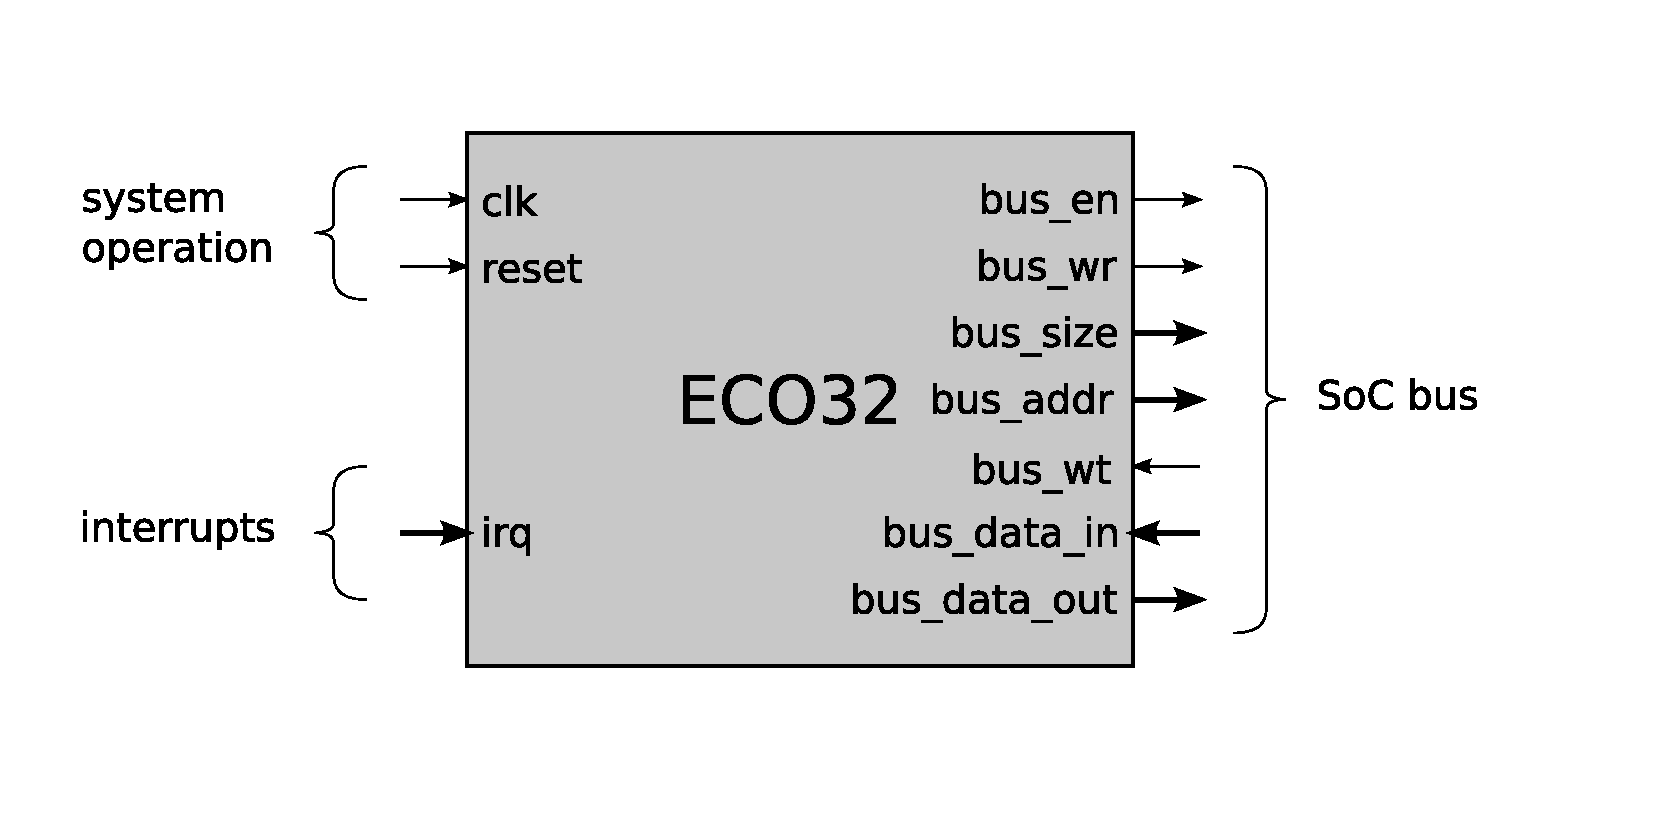
\includegraphics[scale=0.4]{./signals.pdf}
\caption{ECO32 Signal Interface}
\end{figure}

\section{System Operation Signals}
\mylabel{clkreset}

Two system operation signals control the \ecox:
\begin{itemize}
\item The \definition{clk} signal is a positive edge triggered clock signal that controls the timing of the \ecox. Since the \eco is a soft-core processor, minimum and maximum clock frequencies depend on the implementation in an FPGA and cannot be specified in general. The design of the \eco does not impose any particular constraints on the clock frequencies.

All other signals are synchronous to the \name{clk} signal.

\item The \definition{reset} signal is a positive level triggered clock-synchronous reset signal. If the reset is asserted, the \eco is placed into a partly defined reset state, as described in \myref{2}{reset_state} and execution is suspended until the reset is de-asserted. The \eco acts as an inactive master device with respect to the bus interface as long as the reset is asserted.
\end{itemize}

\section{Bus Architecture}
\mylabel{bus}

The \eco can be connected to on-chip devices such as a RAM controller and other devices using a simple SoC bus architecture. The bus uses a synchronous handshake protocol with 32 address bits, 32 data bits, and byte-sized, half-word sized, or word-sized transfers.

Bus operation is divided into \definition{bus cycles}. Each cycle guides a single transfer of a byte, half-word, or word value to or from the \ecox. All transfers are initiated by the \eco and responded to by other devices on the bus. For each transfer, the \eco emits an address that selects both a target device and a location inside that device. It also emits a signal that indicates whether it attempts to read data from that location, or write data to that location. It further emits a signal that indicates the transfer size. Finally, for write operations, the \eco also emits the data to write.

A bus request is responded to by a device with a signal that indicates success of the transfer. If the operation is a read operation, this signal also marks availability of the transferred data. If a certain amount of time passes without any device responding to the request, the transfer is considered failed, and a \name{Bus Timeout Fault} occurs.

\subsection{Bus Timing}

The operation of the SoC bus is synchronous with respect to the system clock. The bus architecture allows to complete a bus cycle with every clock cycle. Peripheral devices may slow down bus operation if they cannot respond fast enough.

A bus cycle begins by the \eco asserting the {\it bus\_en} signal to indicate the start of a transfer. At the same time, it emits the desired values on the {\it bus\_wr}, {\it bus\_size}, {\it bus\_addr}, and {\it bus\_data\_out} lines. The {\it bus\_wr} indicates a read cycle (if de-asserted) or a write cycle (if asserted). The {\it bus\_size} indicates the transfer size, with 10 or 11 indicating a word transfer, 01 indicating a half-word transfer, and 00 indicating a byte transfer. The {\it bus\_addr} is a 32-bit address signal group that selects both a peripheral device and a location in that device. Finally, {\it bus\_data\_out} indicates the transferred data in a write cycle. It is ignored in read cycles. All these signals must keep their value until the clock edge that marks the end of the bus cycle (see below).

The addressed device responds immediately, that is, in the same clock cycle in which the \eco asserted the bus request signals (with no intermediate clock edge), by placing a value on the {\it bus\_wt} line. Each positive clock edge that occurs while {\it bus\_wt} is asserted indicates a wait clock cycle and does not indicate the end of the bus cycle. This allows slower devices to perform internal operations. The device de-asserts {\it bus\_wt} as soon as its internal operations are finished. As soon as a positive clock edge occurs while {\it bus\_wt} is de-asserted, the bus cycle is finished. For read operations, the target device must assert the data to transfer prior to that clock edge, and keep it stable until after that clock edge. The clock cycle following that clock edge is no longer part of the bus cycle, and may witness the start of another bus cycle. Therefore, if the addressed device never asserts its {\it bus\_wt} signal, one bus cycle can be completed in each clock cycle.

If a physical address is emitted on the {\it bus\_addr} lines that is not associated with any device, then the bus itself keeps the {\it bus\_wt} line asserted permanently. This eventually causes the \eco to trigger a \name{Bus Timeout Fault} and stop the bus cycle. A bus timeout is the only event that stops a bus cycle abnormally.

\subsection{Bus Address Map}

The bus architecture places certain restriction on the mapping of physical addresses on the {\it bus\_addr} lines and addresses devices:
\begin{itemize}
\item Addresses in the range 0x00000000 through 0x1FFFFFFF are always associated with a RAM controller. However, only a subrange of these addresses are responded to if the RAM is smaller than 512 MB. RAM may be accessed with (aligned) word, half-word, or byte transfers.
\item Addresses in the range 0x20000000 through 0x2FFFFFFF are always associated with a ROM controller. However, only a subrange of these addresses are responded to if the ROM is smaller than 256 MB. ROM may be accessed with (aligned) word, half-word, or byte transfers.
\item Addresses in the range 0x30000000 through 0x3FFFFFFF are associated with peripheral devices. Their meaning is not further specified. Peripheral device addresses may only be accessed with aligned word transfers.
\item Addresses in the range 0x40000000 through 0xFFFFFFFF are not used. Accesses to these locations will not be responded by any device and cause a \name{Bus Timeout Fault}.
\end{itemize}

\subsection{Bus Sizing}

The {\it bus\_size} signal indicates whether a bus cycle guides a word, half-word, or byte transfer. Access to devices other than RAM or ROM is restricted to word transfers. Half-word and byte transfers on such devices have an unspecified effect.

All word transfers must be aligned to word locations, that is, the lowest two bits of {\it bus\_addr} must be 0. Similarly, half-word transfers must be aligned to half-word locations, that is, the lowest bit of {\it bus\_addr} must be 0. The effect of unaligned transfers is unspecified from the perspective of the SoC bus. The \eco itself prevents such transfers internally and triggers an \name{Illegal Address Fault} instead.

For RAM or ROM locations, a word transfer to or from address $4n$ affects the byte locations $4n$ through $4n+3$ in a big-endian fashion. Similarly, a half-word transfer to or from address $2n$ affects the byte locations $2n$ and $2n+1$ in a big-endian fashion. Write operations change only the affected RAM locations; all other locations are left alone.

During a word transfer, all 32 data lines carry data. During a half-word transfer, only the lower 16 data lines carry transferred data; the others carry unspecified values. During a byte transfer, only the lowest 8 data lines carry data; the others carry unspecified values. Read operations fill the unspecified bits by zero-extending or sign-extending the transferred value. Write operations are either word-sized (in which case there are no unspecified bits), or affect RAM (in which case only 2 or 1 RAM bytes are affected, and the unspecified data lines are ignored).

\subsection{Address Decoding}

During the clock cycle in which the \eco emits a transfer request, the bus decodes addresses by comparing the address sent by the \eco with an individual bit pattern for each device. These patterns are chosen in such a way that at most one comparison succeeds. The corresponding device is \definition{selected} by that address. If no device is selected, the bus asserts the {\it bus\_wt} signal until the \eco detects a timeout.

If a device has been selected, the enable signal for that device is asserted. Thus, the selected device knows it takes part in a transfer by its enable signal. All other devices do not see their enable signal asserted, and thus do not react. A device whose enable signal is de-asserted cannot tell whether a bus transfer involving another device is currently happening.

Since devices whose enable signal is de-asserted do not react to a bus cycle, the bus can safely send the {\it bus\_wr}, {\it bus\_addr}, and {\it bus\_data\_out} to all devices. Devices which have not been selected ignore these values. The same holds true for {\it bus\_size}, but this signal is delivered only to RAM and ROM. All other devices cannot take part in a half-word or byte sized transfer, and implicitly assume word-sized transfers.

Incoming signals from devices are multiplexed by the decoded address. That is, the {\it bus\_wt} and {\it bus\_data\_in} signals arriving at the \eco are those of the selected device. If no device has been selected, {\it bus\_wt} is permanently asserted, and {\it bus\_data\_in} contains a dummy value.

The address lines arriving at each device are a subset of the {\it bus\_addr}. These address lines deliver the \definition{device-local} address. Since each device reacts only if selected, and devices are selected if the address matches a certain bit pattern, only those bits must be delivered that are not yet known by the pattern. Furthermore, delivering those known address bits makes the device unnecessarily sensitive to the positon of its address range in the physical memory map, and thus prevents moving the device to another address range.

The bus may omit further address lines if the corresponding device would ignore them. Most devices need only a tiny subset of their allocated address space, and thus only a subset of the device-local address lines. For example, if the bus uses 12 decoded bits to recognize a device as selected, then that device gets 18 device-local address lines (the lowest two lines are not routed because only aligned word-sized access is allowed). However, a typical device using $8=2^3$ registers would need only 3 device-local address lines. It could then decode the remaining lines and expect them to be 0 (leaving a huge hole in the address map), or ignore them and effectively mirror the 8 registers numerous times to fill the address map. The latter approach requires less hardware resources. However, ignored signal lines usually cause hardware synthesis tools to print warning messages, even if they are bogus as in this case. To prevent these warning messages, the bus may be built such that it does not route the ignored address signals to the device.

By the same reasoning, ignored data signals or other signals can be omitted.

\section{Interrupt Signals}
\mylabel{irqsignals}

The \eco supports 16 interrupt signals that (if accepted) cause a control transfer to the general exception service routine (see \myref{2}{service_routine_address}) and disable interrupt admission temporarily. The interrupt signals need not be associated with other devices on the SoC bus, although this is often the case. The interrupt signals are synchronous, positive level-triggered signals.

Admission of an interrupt is not signalled to the interrupt source automatically. The interrupt service routine must take appropriate action on the SoC bus to cause the corresponding device to de-assert the interrupt signal. Otherwise, as soon as interrupts are enabled again in the \pswx, the still-active interrupt line is recognized again and another interrupt is accepted.

If an asserted interrupt is not immediately accepted by the \eco (e.g. because interrupts are disabled in the \pswx), then the corresponding device can either keep the interrupt signal asserted and be served as soon as the \eco is ready, or de-assert the interrupt signal before the \eco accepts the interrupt and remain unnoticed.

\chapter{Demonstration SoC Project}

This chapter describes a demonstration project that uses the \eco in a SoC design. The project is implemented on an XSA-3S1000 prototyping board form XESS Corp. More information about the prototyping board itself can be found on the XESS homepage, \href{http://www.xess.com}{http://www.xess.com}.

The demonstration project instantiates the \eco inside the Spartan-3 FPGA on the prototyping board and augments it with on-chip controllers for the external hardware on the prototyping board. These controllers are connected to the \eco through the SoC bus. They allow to access the on-board 32 MB SDRAM as the program and data RAM of the \ecox. The flash ROM is connected to the beginning of the peripheral device address space, such that the V bit of the psw selects a base address either in RAM or ROM (see \myref{2}{psw}). Further controllers connected to the SoC bus allow access to a character-based VGA display, PS/2 keyboard, RS232 serial port, and IDE hard disk.

\section{Address Map}

This section describes the mapping of physical addresses to devices in the demonstration project. To access a device directly from a program, direct-mapped virtual addresses can be used that are obtained by adding 0xC0000000 to the physical addresses listed here.

\begin{tabular}{|c|c|c|}
\hline
Physical Address & Virtual Address & Device\\
\hline
00000000$_h$ - 01FFFFFF$_h$ & C0000000$_h$ - C1FFFFFF$_h$ & RAM\\
02000000$_h$ - 1FFFFFFF$_h$ & C2000000$_h$ - DFFFFFFF$_h$ & (unused)\\
20000000$_h$ - 2003FFFF$_h$ & E0000000$_h$ - E003FFFF$_h$ & ROM\\
20040000$_h$ - 2FFFFFFF$_h$ & E0040000$_h$ - EFFFFFFF$_h$ & (unused)\\
30000000$_h$ - 300FFFFF$_h$ & F0000000$_h$ - F00FFFFF$_h$ & Timer\\
30100000$_h$ - 301FFFFF$_h$ & F0100000$_h$ - F01FFFFF$_h$ & Display\\
30200000$_h$ - 302FFFFF$_h$ & F0200000$_h$ - F02FFFFF$_h$ & Keyboard\\
30300000$_h$ - 303FFFFF$_h$ & F0300000$_h$ - F03FFFFF$_h$ & Terminal\\
30400000$_h$ - 304FFFFF$_h$ & F0400000$_h$ - F04FFFFF$_h$ & Disk\\
30500000$_h$ - 3FFFFFFF$_h$ & F0500000$_h$ - FFFFFFFF$_h$ & (unused)\\
40000000$_h$ - FFFFFFFF$_h$ & (not direct-mapped) & (unused)$^*$\\
\hline
\end{tabular}

$^*$these addresses are defined to be permanently unused by the SoC bus architecture.

\section{Interrupt Map}

This section describes the mapping of interrupt numbers (0..15) to devices in the demonstration project. The interupt number specifies both the index of the interrupt signal in the interrupt signal group when connecting the soft-core to other devices, and the number that is placed in the $IEN$ field of the \psw when accepting an interrupt.

\begin{tabular}{|c|c|}
\hline
Interrupt Number & Device\\
\hline
0 & Terminal Sender \#1\\
1 & Terminal Receiver \#1\\
2 & Terminal Sender \#2\\
3 & Terminal Receiver \#2\\
4 & Keyboard\\
5 & (unused)\\
6 & (unused)\\
7 & (unused)\\
8 & Disk\\
9 & (unused)\\
10 & (unused)\\
11 & (unused)\\
12 & (unused)\\
13 & (unused)\\
14 & Timer\\
15 & (unused)\\
\hline
\end{tabular}

\section{RAM and ROM}

The RAM controller connects the \eco to the 32 MB SDRAM chip on the development board. Above 32 MB, the memory map has a hole to allow similar designs with a larger RAM use a compatible memory map. Next comes the ROM controller which connects the \eco to the on-board flash ROM. Only 256 kB of that ROM can be accessed. Note that the ROM also contains the configuration bitstream for the FPGA. The ROM locations for the bit stream are not accessible by the \ecox.

The RAM and ROM are the only devices in the physical address space that may be accessed by half-word and byte transfers. They may contain both program and data. Obviously, the ROM can only contain constant data.

\section{Timer}

The timer is a simple binary counter inside the FPGA that counts clock cycles backwards. Whenever it reaches zero, it is reset to a value specified by a \definition{divisor register} and sets a wrap-around flag. Optionally, this flag generates an interrupt when set. The divisor register thus controls how often the flag is set. 

The \definition{control register} of the timer is used to read or write the wrap-around flag as well as an interrupt enable flag. An interrupt is generated when both the wrap-around flag and the interrupt enable flag are set. The interrupt service routine typically resets the wrap-around flag to de-assert the interrupt signal. Note that the interrupt enable flag is distinct from both the global and the channel-specific interrupt enable flags in the \pswx. 

\begin{tabular}{|c|c|c|c|}
\hline
Bits & 31..2 & 1 & 0\\
\hline
Meaning & (ignored) & Interrupt Enable & Wrap-Around\\
\hline
\end{tabular}

The control register can be accessed at physical address 30000000$_h$ (virtual address F0000000$_h$). The divisor register can be accessed at physical address 30000004$_h$ (virtual address F0000004$_h$).

\section{Display}

The display controller generates a 640x480x60 VGA signal from a 80x30 character matrix, with 8x16 pixels per character. The signal is sent to the VGA port of the prototyping board and can be viewed on a VGA monitor connected to that port. Characters are generated by taking ASCII-encoded characters from the character matrix, converting them to pixels through a character ROM, and applying attributes stored together with the character matrix.

Although the visible character matrix has a size of 80x30, it uses a 128x32 memory internally. These memory locations can be accessed by 128x32 consecutive word locations, stored line by line, at physical addresses 30100000$_h$ through 30100FFC$_h$ (virtual addresses F0100000$_h$ through F0100FFC$_h$). Each word location contains a character code and attributes:

\begin{tabular}{|c|c|c|c|}
\hline
Bits & 31..16 & 15..8 & 7..0\\
\hline
Meaning & (ignored) & Attributes & Character Code\\
\hline
\end{tabular}

The attributes can be subdivided again:

\begin{tabular}{|c|c|c|c|c|c|c|c|c|c|c|}
\hline
Bits & ... & 15 & 14 & 13 & 12 & 11 & 10 & 9 & 8 & ...\\
\hline
Meaning & ... & $BL$ & $R_B$ & $G_B$ & $B_B$ & $I$ & $R_F$ & $G_F$ & $B_F$ & ...\\
\hline
\end{tabular}

The $R_F$, $G_F$, and $B_F$ bits control the base foreground color of the character by enabling the red, green, and blue channels, respectively. If the $I$ bit is set, then all enabled channels are intensified to make the foreground color brighter. The $R_B$, $G_B$, and $B_B$ bits control the color of the background by enabling the red, green, and blue channels, respectively. The $BL$ bit causes the character to \definition{blink}, that is, to become visible and invisible in regular intervals.

The character ROM which contains the pixel patterns for the individual characters cannot be accessed directly.

\section{Keyboard}

The keyboard controller connects the \eco with a keyboard attached to the PS/2 port of the prototyping board. It delivers a stream of \definition{scan codes} from the keyboard which correspond to {\it key press} and {\it key release} events. The decoding of these scan codes is not done by the keyboard controller, but must be done in software instead.

The keyboard controller is accessed by two device registers called the \definition{control register} and the \definition{data register}. When the keyboard controller receives a scancode byte from the keyboard, it stores that byte internally and sets a \definition{ready} flag in the control register. Optionally, the ready flag generates an interrupt: The interrupt signal is asserted if both the ready flag and the interrupt enable flag are set. The corresponding interrupt service routine typically resets the ready flag to de-assert the interrupt signal. The received scancode byte can be read from the data register. Reading from the data register has the side-effect of resetting the ready flag, so the interrupt service routine need not do this manually if it reads from the data register.

The control register can be accessed at physical address 30200000$_h$ (virtual address F0200000$_h$) and has the following layout:

\begin{tabular}{|c|c|c|c|}
\hline
Bits & 31..2 & 1 & 0\\
\hline
Meaning & (ignored) & Interrupt Enable & Ready\\
\hline
\end{tabular}

The data register can be accessed at physical address 30200004$_h$ (virtual address F0200004$_h$) and has the following layout:

\begin{tabular}{|c|c|c|}
\hline
Bits & 31..8 & 7..0\\
\hline
Meaning & (ignored) & Scancode Byte\\
\hline
\end{tabular}

\section{Terminal}

The demonstration project supports a serial terminal connected to the RS232 port of the prototyping board. It also supports a second serial terminal if a modified cable is used: The data transfer lines of the second terminal use the flow control lines of the RS232 port. Using a single terminal with hardware flow control instead of a second terminal is not supported. Also, terminals must currently use a transfer speed of 38400 bauds, a transfer size of 8 bits, 1 start bit, 1 stop bit, and no parity bit.

Each terminal is accessed by four registers: The \definition{receiver control register}, the \definition{receiver data register}, the \definition{sender control register}, and the \definition{sender data register}. These registers can be accessed at the following addresses: 

\begin{tabular}{|c|c|c|}
\hline
Register & Physical Address & Virtual Address\\
\hline
Receiver Control 1 & 30300000$_h$ & F0300000$_h$\\
\hline
Receiver Data 1 & 30300004$_h$ & F0300004$_h$\\
\hline
Sender Control 1 & 30300008$_h$ & F0300008$_h$\\
\hline
Sender Data 1 & 3030000C$_h$ & F030000C$_h$\\
\hline
Receiver Control 2 & 30300010$_h$ & F0300010$_h$\\
\hline
Receiver Data 2 & 30300014$_h$ & F0300014$_h$\\
\hline
Sender Control 2 & 30300018$_h$ & F0300018$_h$\\
\hline
Sender Data 2 & 3030001C$_h$ & F030001C$_h$\\
\hline
\end{tabular}

\subsection{Receiver}

The control register of each receiver contains a \definition{ready flag} that indicates whether a character has been received, and an \definition{interrupt enable flag} to indicate whether the ready flag shall cause an interrupt. The interrupt signal is asserted if both flags are set. Typically, the corresponding interrupt service routine resets the ready flag to de-assert the interrupt signal. The receiver control register has the following layout:

\begin{tabular}{|c|c|c|c|}
\hline
Bits & 31..2 & 1 & 0\\
\hline
Meaning & (ignored) & Interrupt Enable & Ready\\
\hline
\end{tabular}

When a character has been received, it can be read from the receiver data register. Reading a character from the receiver data register has the side-effect of resetting the ready flag. The receiver data register has the following layout:

\begin{tabular}{|c|c|c|}
\hline
Bits & 31..8 & 7..0\\
\hline
Meaning & (ignored) & Received Character\\
\hline
\end{tabular}

\subsection{Sender}

The control register of each sender contains a \definition{ready flag} that indicates whether the sender can accept a character to send, and an \definition{interrupt enable flag} to indicate whether the ready flag shall cause an interrupt. The interrupt signal is asserted if both flags are set. Typically, the corresponding interrupt service routine resets the ready flag to de-assert the interrupt signal. The sender control register has the following layout:

\begin{tabular}{|c|c|c|c|}
\hline
Bits & 31..2 & 1 & 0\\
\hline
Meaning & (ignored) & Interrupt Enable & Ready\\
\hline
\end{tabular}

To send a character, the corresponding data byte must be written to the sender data register. Writing to this register has the side-effect of resetting the ready flag. The sender data register has the following layout:

\begin{tabular}{|c|c|c|}
\hline
Bits & 31..8 & 7..0\\
\hline
Meaning & (ignored) & Character to Send\\
\hline
\end{tabular}

\section{Disk}

The disk controller connects the \eco to an IDE hard disk through the IDE port of the prototyping board. The disk controller simplifies the communication with the disk by hiding the details of the IDE protocol, but in turn allows only simple commands and low transfer speeds.

The disk controller is accessed through the following addresses:

\begin{tabular}{|c|c|c|}
\hline
Location & Physical Address & Virtual Address\\
\hline
Control Register & 30400000$_h$ & F0400000$_h$\\
\hline
Sector Count Register & 30400004$_h$ & F0400004$_h$\\
\hline
Sector Address Register & 30400008$_h$ & F0400008$_h$\\
\hline
Capacity Register & 3040000C$_h$ & F040000C$_h$\\
\hline
(unused) & 30400010$_h$ & F0400010$_h$\\
& ..3047FFFC$_h$ & ..F047FFFC$_h$\\
\hline
Data Buffer & 30480000$_h$ & F0480000$_h$\\
& ..30480FFF$_h$ & ..F0480FFF$_h$\\
\hline
(mirrored data buffer) & 30481000$_h$ & F0481000$_h$\\
& ..304FFFFC$_h$ & ..F04FFFFC$_h$\\
\hline
\end{tabular}

\subsection{Control Register}

The control register is used to read the status of the disk controller, change general control parameters, and initiate actions. It has the following layout:

\begin{tabular}{|c|c|c|c|c|c|c|c|c|}
\hline
Bits & 31 & 30..6 & 5 & 4 & 3 & 2 & 1 & 0\\
\hline
Meaning & DMARQ & (ignored) & INIT & FIN & ERR & WR & IEN & START\\
\hline
\end{tabular}

The DMARQ is a read-only bit that indicates whether the attached disk currently sends a DMA request. This flag can be safely ignored. The INIT flag is a read-only bit that is set to 0 after reset, but turns to 1 as soon as the disk controller has finished initialization. Until the disk is initialized, only the control register should be accessed, and it should only be read to check the status of the INIT flag.

The FIN flag is set to 1 each time the disk controller finishes an operation. The IEN flag can be used to specify whether the FIN flag shall cause an interrupt. The interrupt signal is asserted if both flags are set. Both flags can be changed by writing to the control register. Typically, the corresponding interrupt service routine resets FIN to de-assert the interrupt signal.

The ERR flag is a read-only bit that is either set or reset whenever the disk controller has finished an operation. If set, it indicates an error during the operation.

The WR flag can only be changed while no operation is in progress. It is used to specify whether the disk controller shall perform a read or write operation on the disk.

The START bit is not actually a register. When reading from the control register, it always contains the value 0. Writing a value of 0 to this bit has no effect. Writing a value of 1 initiates the action selected by the WR bit, using the arguments from the sector address and sector count registers.

\subsection{Disk Controller Operations}

An action is initiated by writing a value of 1 to the START bit of the control register. While an action is in progress, the WR bit of the control register, as well as the sector address register and the sector count register cannot be modified. An action transfers sectors from the data buffer to the disk (if WR is set), or from the disk to the data buffer (if WR is reset). The number of transferred sectors is specified by the sector count register. The range of transferred sectors starts at the beginning of the data buffer, and on disk at the sector indicated by the sector address register.

When the transfer is complete, the disk controller resets or sets the ERR flag in the control register, depending on whether the transfer was successful or an error occurred. The disk controller also sets the FIN flag of the control register to indicate completion of the transfer, which causes the interrupt signal to be asserted if the IEN flag is also set.

\subsection{Sector Address, Sector Count, and Capacity}

The sector address register must be set to the number of the first sector on disk to take part in a transfer prior to starting the transfer. Likewise, the sector count register must be set to the number of sectors to transfer prior to starting the transfer. The capacity register is a read-only register that contains the total number of sectors on disk.

\subsection{Data Buffer}

The data buffer has a size of 4096 bytes and thus contains up to 8 sectors. Being located in the device address space, it may only be accessed by word-sized transfers. Since the disk buffer conceptually contains bytes, not words, the word units transferred through the SoC bus comprise the corresponding bytes in a big-endian fashion.

The data buffer should not be accessed while a transfer is in progress.

\chapter{Using the ECO32 in an FPGA Design}

While the \eco is a main component of the demonstration project, it is also a re-usable softcore processor that can be used in arbitrary projects. This chapter explains the necessary steps to use the \eco your next project.



The \eco must also be connected to a RAM to perform any meaningful function. Although it is possible to use the \eco without an attached RAM, such designs would allow only the general-purpose registers to be used for data storage. Typically, the \eco is overkill for such projects, and a smaller processor should be used instead. The RAM can again be implemented as a controller for an off-chip RAM (like in the demonstration project), a block RAM, distributed RAM, or any other kind of memory that satisfies the expectations of a RAM.

The \eco is typically also connected to other on-chip devices to perform its task, such as co-processors, communication controllers, or controllers for off-chip devices. They are connected to the \eco by the SoC bus as well as dedicated interrupt lines. Using the \eco in a custom design implies the design and implementation of such controllers.

Finally, software must be written that is executed by the \ecox. This software is then stored in ROM, pre-loaded into RAM, or stored on an external device and loaded into RAM at run-time. The \eco comes with a tool chain to write such software, comprising an assembler, C compiler, and hardware simulator.

\section{Instantiating the ECO32}

The \eco itself is defined as a synthesizable Verilog module that can be loaded into a project and instantiated as part of a larger design. This larger design must also contain the SoC bus, RAM, ROM, and peripheral devices.

\subsection{Verilog}

The following code instantiates the \eco as part of a surrounding Verilog module:

\begin{verbatim}
cpu mycpu(
  .clk(clk),
  .reset(reset),
  .bus_en(cpu_en),
  .bus_wr(cpu_wr),
  .bus_size(cpu_size[1:0]),
  .bus_addr(cpu_addr[31:0]),
  .bus_data_in(cpu_data_in[31:0]),
  .bus_data_out(cpu_data_out[31:0]),
  .bus_wt(cpu_wt),
  .irq(cpu_irq[15:0])
);
\end{verbatim}

Note how all signals of the enclosing module are prefixed with {\tt cpu\_} to distinguish them from the corresponding signals of other entities on the bus.

\subsection{VHDL}

The following code declares the \eco component in a surrounding VHDL architecture:

\begin{verbatim}
component cpu is
  port (
    clk : in std_logic;
    reset : in std_logic;
    bus_en : out std_logic;
    bus_wr : out std_logic;
    bus_size : out std_logic_vector (1 downto 0);
    bus_addr : out std_logic_vector (31 downto 0);
    bus_data_in : in std_logic_vector (31 downto 0);
    bus_data_out : ou std_logic_vector (31 downto 0);
    bus_wt : in std_logic;
    irq : in std_logic_vector (15 downto 0)
  );
end component;
\end{verbatim}

The following code instantiates that component:

\begin{verbatim}
mycpu : cpu port map (
  clk => clk,
  reset => reset,
  bus_en => cpu_en,
  bus_wr => cpu_wr,
  bus_size => cpu_size,
  bus_addr => cpu_addr,
  bus_data_in => cpu_data_in,
  bus_data_out => cpu_data_out,
  bus_wt => cpu_wt,
  irq => cpu_irq
);
\end{verbatim}

Note how all signals of the enclosing module are prefixed with {\tt cpu\_} to distinguish them from the corresponding signals of other entities on the bus.

\section{SoC Bus}

Using the \eco in a larger design implies connecting it to devices using the SoC bus architecture. This bus must interpret the bus signals from the \eco and transform them to bus signals for the devices. The general bus architecture is explained in \myref{4}{bus}.

\subsection{Instantiation}

Building the bus is easier than it sounds. First, the cpu must be instantiated as explained above. All devices must also be instantiated. Note that a single hardware module may be instantiated multiple times to create multiple similar devices on the bus. For example, the demonstration project instantiates two RS232 serial port controllers from the same Verilog description.

\subsection{Non-Bus Signals}

The {\it clk} and {\it reset} signals must be routed to all instances that need them, including the cpu. All externally available signals must be routed between the ports of the enclosing module and the device instances. For example, in the demonstration project, the {\it r}, {\it g}, {\it b}, {\it hsync}, and {\it vsync} signals must be routed between the ports of the enclosing module and the instance of the character display controller. Finally, the local {\it cpu\_irq} must be assigned individual interrupt signals from the devices.

\subsection{Direct-Routed Bus Signals}

The {\it cpu\_wr} signal is directly routed from the cpu to all peripheral devices. Devices whose enable signal stays de-asserted would ignore the {\it cpu\_wr} signal.

Similarly, {\it cpu\_size} is directly routed to both RAM and ROM. Again, if not selected, these controllers ignore the {\it cpu\_size} signal. Other devices than RAM and ROM implicitly assume word-sized transfers and do not need the {\it cpu\_size} signal.

The write-data lines, {\it cpu\_data\_out}, are directly routed to all devices. However, some devices may need only a subset of these lines if, for example, all acessible device registers are only 8 bits wide. The remaining lines of {\it cpu\_data\_out} are ignored for such devices.

\subsection{Address Decoder}

The {\it cpu\_addr} signal is compared with bit patterns to determine which device is selected (\myref{4}{bus}). This decoder creates one signal per device that is asserted if the device is selected. An example address decoder is shown here that uses 20 device-local address bits (of which the lowest 2 are not routed) for all peripheral devices other than RAM and ROM, a RAM size of 32 MB, and a ROM size of 2 MB.

The address decoder written in Verilog looks like this:
\begin{verbatim}
  wire ram_selected;
  wire rom_selected;
  wire io_selected;
  
  wire device1_selected;
  wire device2_selected;
  
  ...
  
  assign ram_selected =
    (cpu_en == 1 && cpu_addr[31:25] == 7'b0000000) ? 1 : 0;
  assign rom_selected =
    (cpu_en == 1 && cpu_addr[31:21] == 7'b00100000000) ? 1 : 0;
  assign io_selected =
    (cpu_en == 1 && cpu_addr[31:28] == 7'b0011) ? 1 : 0;
    
  assign device1_selected =
    (io_selected == 1 && cpu_addr[27:20] == 7'b00000000) ? 1 : 0;
  assign device2_selected =
    (io_selected == 1 && cpu_addr[27:20] == 7'b00000001) ? 1 : 0;
    
  ...
\end{verbatim}

The address decoder written in VHDL looks like this:
\begin{verbatim}
  signal ram_selected : std_logic;
  signal rom_selected : std_logic;
  signal io_selected : std_logic;
  
  signal device1_selected : std_logic;
  signal device2_selected : std_logic;
  
  ...
  
  ram_selected <=
    cpu_en when cpu_addr(31 downto 25) = "0000000" else '0';
  rom_selected <=
    cpu_en when cpu_addr(31 downto 21) = "00100000000" else '0';
  io_selected <=
    cpu_en when cpu_addr(31 downto 28) = "0011" else '0';
    
  device1_selected <=
    io_selected when cpu_addr(27 downto 20) = "00000000" else '0';
  device2_selected <=
    io_selected when cpu_addr(27 downto 20) = "00000001" else '0';
    
  ...
\end{verbatim}

The {\it \_selected} lines for the individual devices are directly routed to the enable ports of the corresponding devices. The local address ports of each device are connected with the remaining address bits. For example, the local address ports of device1 are connected with cpu\_addr$_{19..0}$. A subset of those address lines may be used if the device ignores the remaining lines.

\subsection{Response Signal Multiplexer}

The response signals from the devices, {\it device$^*$\_wt} and {\it device$^*$\_data\_out}, are multiplexed by the {\it cpu\_addr} before delivered to the \eco as {\it cpu\_wt} and {\it cpu\_data\_in}. This way, the \eco always sees the response signal of the selected device.

The response signal multiplexer written in Verilog looks like this:
\begin{verbatim}
  assign cpu_wt =
    (ram_selected == 1) ? ram_wt :
    (rom_selected == 1) ? rom_wt :
    (device1_selected == 1) ? device1_wt :
    (device2_selected == 1) ? device2_wt :
    1;
  assign cpu_data_in =
    (ram_selected == 1) ? ram_data_out :
    (rom_selected == 1) ? rom_data_out :
    (device1_selected == 1) ? device1_data_out :
    (device2_selected == 1) ? device2_data_out :
    32'h00000000;
\end{verbatim}

The response signal multiplexer written in VHDL looks like this:
\begin{verbatim}
  cpu_wt <=
    ram_wt when ram_selected = '1' else
    rom_wt when rom_selected = '1' else
    device1_wt when device1_selected = '1' else
    device2_wt when device2_selected = '1' else
    '1';
  cpu_data_in <=
    ram_data_in when ram_selected = '1' else
    rom_data_in when rom_selected = '1' else
    device1_data_in when device1_selected = '1' else
    device2_data_in when device2_selected = '1' else
    "00000000000000000000000000000000";
\end{verbatim}

\section{RAM and ROM Controllers}

After reset, the \pc is set to virtual address E0000000$_h$ (physical address 20000000$_h$) and therefore points to the first location in ROM. There are several ways to connect a ROM to this address, for example:
\begin{itemize}
\item implement a controller for an off-chip ROM. For example, the demonstration project connects an address range starting at physical address 20000000$_h$ to a controller for the flash ROM on the development board.
\item connect a range of addresses starting at physical address 20000000$_h$ to one or more block RAMs configured as ROMs
\item connect a range of addresses starting at physical address 20000000$_h$ to distributed ROM
\item implement logic that emits a jump instruction to virtual address C0000000$_h$ which is direct-mapped to RAM. This solution requires that RAM is pre-initialized with a program to jump to.
\end{itemize}

The physical address range 00000000$_h$ through 1FFFFFFF$_h$ is associated with RAM. There are several ways to connect a RAM:
\begin{itemize}
\item implement a controller for an off-chip RAM. For example, the demonstration project connects an address range starting at physical address 00000000$_h$ to a controller for the SDRAM on the development board.
\item connect a range of addresses starting at physical address 00000000$_h$ to one or more block RAMs.
\item connect a range of addresses starting at physical address 00000000$_h$ to distributed RAM
\end{itemize}

\section{Peripheral Controllers}

The \eco can be connected to arbitrary FPGA designs to control the operation of these designs or perform computations on behalf of a larger design. For example, it can be connected to an RS232 transceiver to communicate with other physical devices. The range of possible FPGA designs that can cooperate with the \eco shall not be discussed here. Instead, this section explains {\it how} to make the connection.

The primary means of communication between the \eco and other devices is the SoC bus. The bus provides means for basic {\it read} and {\it write} operations, but does not define the meaning of these operations. This section gives some suggestions how to use these operations as part of a larger design.

\subsection{Device Address Map}

Peripheral controllers must be connected to physical addresses in the range 30000000$_h$ through 3FFFFFFF$_h$ (virtual addresses in the range F0000000$_h$ through FFFFFFFF$_h$). The subdivision of this range across different devices is not specified and can be chosen freely. This allows the use of both many devices with a small address range and few devices with a large address range in the same design.

\subsection{Device-Local Addresses}

The device-local address contains those address bits of the 32 bus address lines that have not been decoded to select a specific device. The meaning of the device-local address was clear in the context of a RAM or ROM. For peripheral controllers, there is more freedom. A device-local address in such a controller can select a device register, or a location in a device-specific RAM, or even a location that does not actually store values.

In general, the device-local address is a piece of information that is always transferred to the target device, whether in read operations or write operations. For read operations, it specifies what kind of data is requested. For write operations, it tells the device what to do with the data.

A typical way to interpret a device-local address is by building an address decoder. Much like the coarse address decoder found in the bus itself, it compares the device-local address with bit patterns to generate enable signals for individual components in a device, and to multiplex response data from individual components.

\subsection{Device Registers}

The most common construct to connect to the bus is a register. Such registers keep control values and data for the operation of a device. Registers can have any size from 1 to 32 bits. Larger registers cannot be fully accessed in a single bus operation and must be wired to the bus as multiple separate registers, typically at different device-local addresses.

Write data coming from the \eco is wired to the data-in port of the register. Read data is generated directly from the data-out port of the register. The device-local address decoder then multiplexes between read data from different registers. Finally, the device-local address decoder asserts the clock enable signal for the register if both the device-specific bus enable signal is asserted and the device-local address selects this specific register. The {\it wait} signal of the bus can be tied low for registers, since they do not introduce any delays.

The current value of the register is not only delivered as read data to the \ecox, but is also used by the device itself. In some cases, the value of the register is modified by the device such that the new value can be read by the \ecox. There are various ways in which a register value can influence the operation of a device, which cannot all be described here. For example, the value can consist of control fields that determine the operation mode of the device. Registers can also contain data to be sent to external targets by the device, or data that was received from external sources.

\subsection{Device RAM}

Some devices may use the device-local address to access a RAM, just like the main RAM does. Device RAM is different from regular RAM in the sense that it must be accessed only by word-sized transfers. Typically, device RAM is accessed by the \eco only in block transfers to and from regular RAM.

Device RAM is typically used for large data blocks to be sent or received by a device. For example, the disk controller of the demonstration project uses a 4kB RAM for data that is transferred to and from disk. The bus architecture demands that this RAM be accessed as 1k words, and never as 2k half-words or 4k bytes. Another use for device RAM would be the storage of program and data of a co-processor.

Device RAM can be easily implemented by connecting the data-in, data-out, and device-local address to a block RAM of the FPGA. The wiring of the {\it wait} and {\it enable} signals is slightly more complex due to the block RAM being only synchronously readable. A read operation requires two clock cycles, so the bus {\it wait} signal must be asserted in the first of those cycles, and de-asserted in the second one. Write operations take only a single clock cycle, and the {\it wait} signal must stay de-asserted.

This behaviour can be implemented easily. First, the bus enable signal is connected directly to the clock enable port of the block RAM. This causes the block RAM to finish writing in one clock cycle, and to read data at the edge between the first and second clock cycle of a read operation. Since the bus enable signal stays asserted until the bus cycle is complete, it also causes the block RAM to read again at the end of the second clock cycle, but from the same address, and the resulting value is ignored anyway. Only the value read after the first clock cycle is used.

The behaviour of the wait signal is also simple. For write operations, it must stay de-asserted. For read cycles, it must be asserted for one clock cycle, then de-asserted for one clock cycle. A simple state machine with two states takes care of this.

\subsection{FIFO Queues}

A device-local address can select a FIFO queue that delivers or consumes data. Typically, a single device-local address selects either a read queue or a write queue, although it is possible to connect one queue of either type to the same address (and distinguish between them by the bus {\it write} signal).

FIFO queues have the special property that successive values are read from or written to the same device-local address. When writing data to a FIFO queue, the order in which values are written determines the order in which they are handled. When reading data from a FIFO queue, the order in which values arrive is the order in which the \eco should handle them. FIFO queues are typically associated with a communication stream.

\subsection{Address Registers}

It is possible to associate a single device-local address with multiple target registers. In such designs, a separate source for address bits is needed besides those coming from the bus. These additional address bits are decoded to generate enable signals for the target registers and to multiplex data read from them.

A separate register at another device-local address, called an \definition{address register}, is used to store these additional address bits. First, the program running on the \eco writes the address of the intended target register into the address register. Then, it writes to or reads from the multiplexed device-local address to access the target register itself.

\subsection{Trigger Signals}

A device sometimes needs a signal telling it to start some action. For example, the disk controller in the demonstration project is first configured by writing appropriate values into its control registers, then triggering the start of the configured operation. Such a trigger need not store any values, and thus need not be backed by a physical register. Instead, the trigger signal causes a transition in the state machine of the device that begins the operation.

A simple design would take the enable signal of that device local address as the trigger signal. This enable signal is in turn asserted if both the bus {\it enable} signal is asserted and the correct device-local address is supplied. The \eco starts the operation by reading from or writing to that address. More sophisticated designs could take the value of the {\it write} signal into account, such that only writing starts the operation, or even look for writing a 1 bit to a specific bit position. This is important if the trigger signal is grouped together with other values at the same device-local address.

\subsection{Bus-Mapped Logic}

It is possible to implement an often-used boolean function in hardware and connect it directly to the bus, with no intermediate registers. This function can have as many input bits as it has device-local address bits, and up to 32 output bits which it connects to its data-out port. The \eco can access the boolean function block by encoding both the base address of the function block device and the input bits for the function in a 32-bit physical address, then reading from that address. The resulting value is the result of the function.

\section{Interrupts}

Some devices need to signal to the \eco that some event has occurred without the \eco specifically asking for it. For example, the RS232 controller of the demonstration project must signal to the eco when a character has been received, without the \eco constantly asking the RS232 controller if characters are available. {\it Interrupts} are used for this.

The \eco supports up to 16 level-triggered interrupt signals. A device asserts its interrupt signal when it needs attention from the \ecox. The \eco then performs whatever action is needed for the device. Specifically, it performs some action that causes the device to de-assert its interrupt signal. Interrupt handling from the perspective of the \eco has been described before. This section explains interrupts from the perspective of the peripheral devices.

A straightforward way to implement interrupts in a device is to use a 1-bit register that can be set or reset both by the device and the \eco (via the bus). The value of this register is taken as the interrupt signal. When the device detects an event that is worth an interrupt, it sets the register to 1. This causes the \eco to enter its interrupt service routine, where it deals with the event. The service routine also writes a 0 to the register via the bus to de-assert the interrupt signal, such that it can leave the service routine without generating another interrupt.

A more sophisticated design is used in the demonstration project. This uses another 1-bit register that acts as an {\it interrupt enable} and is written to solely by the \ecox. The demonstration project groups both 1-bit registers into a 2-bit register at a single device-local address. The interrupt signal is generated by ANDing both registers. This allows to disable interrupt generation in the device itself. Normally, the \eco does not need such a design because it can disable each interrupt channel individually through the $IEN$ field of the \pswx. However, more complex designs may involve more than 16 interrupt-capable devices and require that multiple devices share a single interrupt signal. In that case, disabling interrupts per-device, and not per-channel, is a useful feature.

\chapter{Tool Chain}
\label{tool_chain}

The \eco comes with tool programs that allow the development of software for it. The software package currently includes an assembler, C compiler, instruction-level simulator, and various support tools.

\section{Assembler ({\tt asld})}

The {\tt asld} tool assembles and links a set of files written in a custom assembler format to produce an executable binary. The binary uses either a custom segmented binary format, or a raw dump of the code and data segments. It is currently impossible to separate the assembler and linker stages.

\subsection{Command Line Interface}

{\bf Synopsis:}\\
{\tt asld [options] file [files ...]}

The {\tt asld} tool reads all files and interprets them according to a custom assembler format described below. The files are then assembled in the order specified in the command line to produce an executable. Various options control this process:
\begin{itemize}
\item {\tt \bf -h}: Generates a {\it headerless} binary that contains only a raw dump of the code and data sections in direct sequence, without any header.
\item {\tt \bf -o \it objfile}: Specifies the name of the generated binary.
\item {\tt \bf -m \it mapfile}: Specifies the name of a {\it map file} that is created in addition to the output binary. This map file contains a listing of the final global symbol table.
\item {\tt \bf -rc \it Address}: Specifies the (virtual) start address of the code section. This affects the target location of symbols in that section. It does not affect the position of the code section within the generated binary file. If this option is not specified, the start address of the code section defaults to 0.
\item {\tt \bf -rd \it Address}: Specifies the (virtual) start address of the data section. This affects the target location of symbols in that section. It does not affect the position of the data section within the generated binary file. If this option is not specified, the start address of the data section defaults to the end of the code section, rounded up to 4k page boundaries.
\item {\tt \bf -rb \it Address}: Specifies the (virtual) start address of the BSS section. This affects the target location of symbols in that section. It does not affect the position of the BSS section within the generated binary file. If this option is not specified, the start address of the BSS section defaults to the end of the data section, without any rounding.
\end{itemize}

\subsection{Assembling Model}

The assembler maintains the following state variables:

\begin{itemize}
\item Three sections, called {\it code}, {\it data}, and {\it BSS}. Each section consists of a byte array starting at index 0. The number of bytes in this array is the {\it size} of the section. The only way to modify a section is to append bytes at the end. Note that while the BSS is treated like the other sections, its contents are not written to the output file.
\item A symbol table. Each entry of this table maps an identifier to a (section, index) pair and thus points to a specific location in a specific section. As a special rule, the section of a symbol can be the special {\it absolute} section, meaning that the symbol is not relative to any defined section and is thus not relocated. The symbol table is split into a {\it local} and a {\it global} part for file-local and cross-file symbols (see below).
\item A {\it current section}, which is one of the three sections defined above. The special {\it absolute} section cannot be the current section.
\item Various control parameters.
\end{itemize}

At the beginning of the assembly process, all three sections are empty, the global symbol table is empty, the current section is the code section, and the control parameters are set to their default values. The assembler then begins to consume the input files one by one. For each file, the following steps are performed:
\begin{itemize}
\item Clear the local symbol table.
\item Set the current section to the code section (<-- not sure about this, but would make sense)
\item Reset some of the control parameters to their default values.
\item Process the file as described in the next section.
\end{itemize}

After all files have been consumed, symbols are relocated and back-patched: First, the start location of each section is determined either automatically or by the {\tt -r}$^*$ command-line switches. The {\it relocated position} of a symbol is obtained by adding the start address of the symbol's section to the location of the symbol within its section. Symbols in the special {\it absolute} section use their section-local position as the relocated position, which is equivalent to saying that the start address of the {\it absolute} section is 0. The assembler then scans through all references to symbols in the assembled code and inserts the relocated address.

Finally, the output binary is generated by writing the header (containing the section sizes; only if {\tt \bf -h} has not been specified) and the contents of the code and data sections.

\subsection{Input Format}

An assembler input file is a sequence of {\it labels}, {\it instructions}, and {\it processing directives}. Each of them modifies the assembler state defined in the previous section:
\begin{itemize}
\item A {\it label} creates an entry in the local symbol table. It is specified as an identifier, followed by a colon character. This identifier names the entry that is created in the local symbol table. The target location of the symbol is the current section and the current location in that section.
\item An instruction is a simple identifier that is one of the instruction mnemonics of the \ecox, followed by the operands of that instruction. For convenience, the non-immediate mnemonic may be used with an immediate operand to specify the immediate instruction, such as ADD for ADDI. Register operands are specified by a dollar sign, followed by the number of the register. Immediate operands are specified as a simple number. Jump targets are specified by a label identifier. Operands must be comma-separated. The specified instruction is assembled at the current location in the current section (usually, but not necessarily, the code section).

The control parameters may be set up to allow {\it synthesized instructions}. These look like single instructions in the input file, but are actually assembled as short instruction sequences. Synthesized instructions exist purely for convenience when writing assembler code manually.
\item A processing directive starts with a dot, followed by the name of the directive. The following directives exist:
\begin{itemize}
\item {\tt \bf .syn}: Enables synthesized instructions.
\item {\tt \bf .nosyn}: Disables synthesized instructions.
\item {\tt \bf .code}: Makes the code section the current section.
\item {\tt \bf .data}: Makes the data section the current section.
\item {\tt \bf .bss}: Makes the BSS section the current section.
\item {\tt \bf .export}: Creates a global symbol table entry from a local one. This directive expects a list of symbol names, all of which are exported.
\item {\tt \bf .import}: Creates a local symbol table entry by importing a global symbol. The corresponding global symbol must be defined in past or future assembler input within the same assembler run, otherwise an error occurs. This directive expects a list of symbol names, all of which are imported.
\item {\tt \bf .align}: Inserts padding bytes for half-word or word alignment. Formally, this directive expects a number argument which must be a power of 2, and inserts zeroed bytes into the current section until the current position in the current section is a multiple of that number. The result is undefined if the specified number is not a power of 2.

This directive is typically used directly before half-word or word sized variables are emitted, because access to these variables must be aligned to the access size. As an example, ``{\bf align 2}'' inserts a zeroed byte if the current position is an odd position, and thus aligns the current position to generate a half-word variable. Similarly, ``{\bf align 4}'' aligns the current position for word-sized variables.
\item {\tt \bf .space}: This directive expects a number argument and emits that number of zeroed bytes to the current section.
\item {\tt \bf .locate}: This directive expects a number argument and emits zeroed bytes to the current section until the current position in the current section is equal to that number. The specified number {\it must not} be less than the current position in the current section, otherwise the {\tt asld} will crash.
\item {\tt \bf .byte}: Emits a single byte to the current section whose value is the argument to this directive.
\item {\tt \bf .half}: Emits two bytes to the current section whose value is the argument to this directive in big-endian representation. The {\tt .half} directive can emit half-words at unaligned memory locations, however, the \eco will not be able to read then a half-word units.
\item {\tt \bf .word}: Emits four bytes to the current section whose value is the argument to this directive in big-endian representation. The {\tt .word} directive can emit words at unaligned memory locations, however, the \eco will not be able to read then a word units.
\item {\tt \bf .set}: This directive expects an identifier and numeric value as its arguments, and creates a symbol in the special {\it absolute} section with that identifier and value.
\end{itemize}
\end{itemize}

\subsection{Output Format}

The output format of {\tt asld} is a single file that consists of a {\it header} and a {\it body}. If the {\tt \bf -h} option is specified, the header is omitted. The header contains the following fields in big-endian byte order:

\begin{itemize}
\item Magic Number (4 bytes): Must be 3AE82DD4$_h$.
\item Code Section Size (4 bytes)
\item Data Section Size (4 bytes)
\item BSS Section Size (4 bytes)
\end{itemize}

The body contains the contents of the code and data sections in direct sequence, without any padding in between. It is the responsibility of the loader to ensure that these sections are loaded to the (virtual) section start addresses determined at assembly time. The BSS conceptually contains only zeroed bytes, and thus isn't stored in the binary file. It is the responsibility of the loader to ensure that the contents of the BSS are actually zeroed.

\section{C compiler ({\tt lcc})}

The {\tt lcc} tool is a C compiler, based on the LCC source code, for ANSI C (C89). Currently, it must be used in conjunction with the {\tt asld} tool to compile a whole project at once, because there is no object format for individual compiled C sources. Assembler and C sources can be mixed in a compiler run, and will be assembled in exactly the order specified at the command line. Unless overridden, the generated object file is a simple segmented format.

\subsection{Command Line Interface}

LCC supports various switches on the command line that can be viewed by running it without arguments. The general synopsis is:

{\tt lcc [option | file] ...}

Each file is either a C or assembler input file. The input files are assembled in the specified order.

The {\tt \bf -W} argument is a generic extension mechanism for command-line arguments. Only the most important uses of this mechanism will be explained here:
\begin{itemize}
\item {\tt \bf -Wo-kernel}: Sets the start address of the code section to C0000000$_h$ as if {\tt \bf -Wl-rc -Wl0xC0000000} had been specified, and prevents linking to the standard library. Since there is no useful standard library yet, this switch must be specified. Alternatively, compilation can be done using {\tt \bf -s} and assembly/linking be done in a separate step, which has the same effect.
\item {\tt \bf -Wl-m -Wl}{\it mapfile}: Generates a {\it map} file that lists the entities assembled to the output file.
\item {\tt \bf -Wl-h}: Generates a {\it headerless} output file. The output file does not contain the simple segmented output format. Instead, it only contains the contents of the code and data section in direct sequence.
\item {\tt \bf -Wl-rc -Wl0x}{\it Address}: Specifies the start address of the code section. This affects the (jump) addresses within the code that is ultimately written to the output file.
\item {\tt \bf -Wl-rd -Wl0x}{\it Address}: Specifies the start address of the data section. This affects the (load/store) addresses within the code that is ultimately written to the output file.
\item {\tt \bf -Wl-rb -Wl0x}{\it Address}: Specifies the start address of the BSS section. This affects the (load/store) addresses within the code that is ultimately written to the output file.
\end{itemize}

\subsection{Data Types}

The C compiler uses the following bit sizes for the C data types:

\begin{tabular}{|c|c|}
\hline
long & 32\\
int & 32\\
short & 16\\
char & 8\\
pointer & 32\\
\hline
\end{tabular}

\subsection{Register Allocation}

The C compiler assigns a fixed purpose to each register index:

\begin{tabular}{|c|l|}
\hline
Index & Meaning\\
\hline
0 & tied to value 0 by the hardware\\
\hline
1 & reserved as an auxiliary register for use by the assembler\\
& (not used by the compiler)\\
\hline
2,3 & function return value\\
\hline
4..7 & function arguments\\
\hline
8..15, 24, 25 & caller-save local value, to be used for temporary results\\
\hline
16..23 & callee-save local value, to be used for local variables\\
\hline
26..28 & reserved for OS kernel\\
& (not used by the compiler)\\
\hline
29 & stack pointer\\
\hline
30 & reserved for interrupt return address \\
& (not used by the compiler)\\
\hline
31 & function return address\\
\hline
\end{tabular}

\section{Simulator}

...

\section{\tt bin2exo}

The {\tt bin2exo} tool converts a binary file to a {\tt .exo} file to be loaded into the flash ROM. The {\tt .exo} file contains exactly the byte sequence stored in the binary file, converted to Motorola S-Records, without any headers, stripping, or byte swapping. The start address at which the data is placed in ROM can be specified via the command line.

\subsection{Command-Line Options}

Synopsis:
\begin{itemize}
\item[] {\tt bin2exo <load address, hex> <input file> <output file>}
\end{itemize}

The {\it load address} specifies the first address in the flash ROM, specified as a hexadecimal number, that is occupied by the contents of the {\it input file}. This file is converted to Motorola S-Records, which are stored in the {\it output file}, which presumably is a {\tt .exo} file.

\subsection{Generating a Boot ROM}

The {\tt bin2exo} tool can be used to convert a binary file to a boot ROM for the \ecox. To do so, the binary file must be converted to a {\tt .exo} file with start address 0 and loaded into the flash ROM using the {\tt GXSLOAD} tool. This maps the contents of the binary file to physical address 20000000$_h$ (virtual address E0000000$_h$) upwards, and thus causes the \eco to interpret the contents of the file as raw instructions after reset.

Note that while neither the binary file nor the {\tt bin2exo} tool or the {\tt .exo} file have a notion of a byte order, using the file as a boot image causes the \eco to access its contents in a big-endian fashion, just as expected. This is the result of various intermediate steps, such as the {\tt GXSLOAD} program, the parallel interface to the XSA board, the CPLD configuration, the byte order of the flash ROM itself, and the ROM interface that connects the flash ROM to the SoC bus. Not all of these steps are well-documented, and no assumptions should be made about the intermediate byte order if this chain is broken.

\section{\tt bit2exo}

The {\tt bit2exo} tool converts a Xilinx {\tt .bit} file to a {\tt .exo} file that can be loaded into the Flash ROM to configure the FPGA on startup. It is important to use {\tt bit2exo}, and not {\tt bin2exo} for this job, because the {\tt .bit} file contains headers that must be stripped from the actual bit stream. The start address at which the bit stream is placed in ROM can be specified in hexadecimal via the command line, and should be the start address of one of the four ROM quadrants:

\begin{tabular}{|c|c|}
\hline
ROM Quadrant & Start Address\\
\hline
0 & 000000$_h$ \\
\hline
1 & 080000$_h$ \\
\hline
2 & 100000$_h$ \\
\hline
3 & 180000$_h$ \\
\hline
\end{tabular}

Due to the architecture of the \ecox, quadrant 0 usually contains the boot loader code and therefore cannot be used for the FPGA configuration. By placing the configuration in quadrant 3, quadrants 0 through 2 can be usd as a continguous program ROM. {\bf Note:} Do not forget to place the jumpers on the FPGA board to tell the FGPA from which quadrant to load its configuration.

\subsection{Command-Line Options}

Synopsis:
\begin{itemize}
\item[] {\tt bin2exo <load address, hex> <input file> <output file>}
\end{itemize}

The {\it load address} specifies the first address in the flash ROM, specified as a hexadecimal number, that is occupied by the contents of the bit stream found in the {\it input file} after stripping all headers. The bit stream is converted to Motorola S-Records, which are stored in the {\it output file}, which presumably is a {\tt .exo} file.




\chapter{Implementation Notes}

\section{XSA-3S1000 SDRAM Controller}

\subsection{Refresh}

SDRAM cells must be refreshed repeatedly to keep their value. The SDRAM knows three methods of refreshing cells:
\begin{itemize}
\item {\it Self-Refresh}: The SDRAM is detached from the FPGA and refreshes all cells periodically. No other functions can be used while self-refresh is in progress. This mode is not used by the current controller.
\item {\it Auto-Refresh}: The SDRAM keeps an internal row counter purely for refreshing. The {\it auto-refresh} command refreshes the current row and increases the counter. This mode is used by the current controller to refresh all rows periodically. The refresh circuit is independent from the RAM access interface and refreshes all rows periodically regardless of the memory access pattern of the client.
\item {\it Manual Refresh}: Manual refresh of a row occurs when that row is activated. Implicit manual access occurs when a row is activated for reading or writing, and may occur depending on the access pattern of the client. It is not exploited though. Explicit manual refresh occurs when a row is opened purely to refresh it, and is not used by the current controller.
\end{itemize}

An access arbiter is required to interleave access to the SDRAM by the refresh circuit and by the actual memory access interface. In the current implementation, an access burst in progress is allowed to finish, then refreshing gets absolute priority. The actual implementation keeps a counter of pending rows to refresh and a timer. Whenever the timer runs out, the number of rows to refresh is increased by one. Whenever the number of rows to refresh is greater than zero {\it and} the memory access interface does not actually access the SDRAM, a row is refreshed and the number of rows to refresh is decreased by one. This scheme allows ``alarms'' from the refresh timer to accumulate while a burst is in progress, and perform them all in sequence when the burst is completed.

\subsection{States}

After initialization, the SDRAM has three persistent states:
\begin{itemize}
\item Idle (pre-charged): The row data register of the SDRAM is pre-charged and ready to activate a row. This state can also be used to set the mode register or to activate auto-refresh.
\item Row Active: A row has been loaded into the row data register. Either a transfer of data to or from this row can be started, or the row data register can be pre-charged to activate another row. Minimum delays must be obeyed to ensure that the value from the row data register can be written back to the DRAM array, either unchanged (for manual refresh) or changed (for actually writing data to the DRAM array).
\item Transfer: Reading or writing data to or from the row data register. The SDRAM supports an auto-precharge mode (???).
\end{itemize}

It also has transitional states to represent the non-immediate transition between the persistent states:
\begin{itemize}
\item Mode Register Accessing: A transition from {\it Idle} to {\it Idle}. Represents the time to store a new value in the mode register.
\item Activating: A transition from {\it Idle} to {\it Active}. Represents the time to load a row from the DRAM array. The time to complete this transition is $t_{RCD}$, the RAS-to-CAS delay (so called because the activation of a row is signalled by $\overline{RAS}$ going low, and access to a memory cell is signalled by $\overline{CAS}$ going low.)
\item Precharging: A transition from {\it Active} to {\it Idle}. Represents the time to pre-charge the row data register of the SDRAM.
\end{itemize}

\subsection{Clocking}

Based on current knowledge (!!!)

The explanation in this section assumes that the SDRAM controller uses registers for all data signals both at the input and output pins, without any logic in between, clocked by the internal FPGA clock.

The FPGA uses a DCM to generate the clock for the SDRAM. The input clock to the DCM is the global clock of the FPGA circuits. The output clock is fed through an output buffer to the SDRAM. The SDRAM feedback clock is fed to an IBUFG and to the feedback input of the DCM.

How this works: The path from the DCM output to the SDRAM serves two purposes. The first purpose is to act as a clock source at the SDRAM clk pin. The SDRAM works synchronous to this clock source: It samples its inputs when a clock edge occurs at the clk pin, and changes its outputs in such a way that setup and hold timing is not violated with respect to the clk pin.

When the SDRAM tries to send data to the FPGA, it asserts the data signals between two clock edges, such that the data is stable on each clock edge. Data and (feedback) clock signals have comparable delays between their source at SDRAM pins and their destination inside the FPGA. These delays consist of PCB trace delays, input buffer delays, and FPGA-internal delays. Sicne the delays are comparable, the FPGA could in theory use the clock signal coming from the SDRAM to clock registers which sample the data signals coming from the SDRAM without violating setup/hold timing.

This is where the second purpose of the DCM comes in: The feedback clock from the SDRAM is kept in phase with the FPGA-internal clock, meaning that the FPGA can as well use the internal clock to sample the data signals from the SDRAM. The DCM therefore ensures that reading data from the SDRAM works without problems using the internal clock.

Writing data to the SDRAM works by keeping the clock frequency low enough: The internal FPGA registers load their new values when a clock edge occurs inside the FPGA, i.e. one SDRAM-to-FPGA signal delay after the clock edge occurs at the SDRAM. The new values are available after the clock-to-out delay of the FPGA registers. They arrive at the SDRAM one FPGA-to-SDRAM delay later, and must respect the setup timing of the SDRAM. The sum of all these delays must be less than the clock period.

The net effect is that clock edges occur in an alternating fashion in the FPGA and in the SDRAM. This leaves roughly half a clock period to transfer a signal to or from the SDRAM. For example, a read command with a CAS latency of 3 is explained as the data being available three clock periods after the CAS. Executing this command works as follows (timing measured in clock periods):
\begin{itemize}
\item 0: a CAS command is loaded into the FPGA output registers with an FPGA clock edge
\item 0.5: The SDRAM samples its inputs at an SDRAM clock edge and recognizes the command
\item 1.5: ... working ...
\item 2.5: ... working ...
\item 3.3: The SDRAM asserts data outputs roughly here
\item 3.5: The SDRAM guarantees valid data at this SDRAM clock edge
\item 4.0: The FPGA samples the data signals at this FPGA clock edge
\end{itemize}

Depending on the clock frequency, the distance between clock edges may shift: The delay from an SDRAM clock edge to the next FPGA clock edge is determined by the signal delay, and is therefore independent from the clock frequency. The delay from an FPGA clock edge to the next FPGA clock edge is simply the remainder of the clock period. With the clock period long enough, the delay from an FPGA clock edge to the next SDRAM clock edge is long enough for signals to be transmitted. Signals back to the FPGA experience the same delay as the feedback clock and therefore always arrive early enough.

\begin{thebibliography}{sotief}

\bibitem{tanenbaum}
Andrew S. Tanenbaum, Albert S. Woodhull. 
{\it Operating Systems: Design and Implementation}.
second edition, Prentice-Hall, 1997

\bibitem{lions}
John Lions.
{\it Lions' Commentary on UNIX 6th Edition with Source Code}.
Peer-to-Peer Communications, 1996

\bibitem{bach}
Maurice J. Bach.
{\it The Design of the UNIX Operating System}.
Prentice-Hall, 1986

\bibitem{c_programming_language}
Brian W. Kernighan, Dennis M. Ritchie.
{\it The C Programming Language}.
second edition, Prentice-Hall, 1988

\bibitem{retargetable_c_compiler}
Christopher W. Fraser, David R. Hanson.
{\it A Retargetable C Compiler: Design and Implementation}.
Addison-Wesley, 1995

\bibitem{standard_c_library}
P. J. Plauger.
{\it The Standard C Library}.
Prentice Hall P T R, 1992

\bibitem{see_mips_run}
Dominic Sweetman.
{\it See MIPS Run}.
Morgan Kaufmann, 1999

\bibitem{mips_risc_architecture}
Gerry Kane, Joe Heinrich.
{\it MIPS RISC Architecture}.
Prentice-Hall, 1992

\bibitem{dlx}
Philip M. Sailer, David R. Kaeli.
{\it The DLX Instruction Set Architecture Handbook}.
Morgan Kaufmann, 1996

\bibitem{patterson_henessy}
David A. Patterson, John L. Hennessy.
{\it Computer Organization \& Design: The Hardware/Software Interface}.
second edition, Morgan Kaufmann, 1998

\bibitem{henessy_patterson}
John L. Hennessy, David A. Patterson.
{\it Computer Architecture: A Quantitative Approach}.
second edition, Morgan Kaufmann, 1996

\bibitem{ashenden}
Peter J. Ashenden.
{\it The Designer's Guide to VHDL}.
Morgan Kaufmann, 1996

\bibitem{moorby}
Donald E. Thomas, Philip R. Moorby.
{\it The Verilog Hardware Description Language}.
fifth edition, Kluwer Academic Publishers, 2002

\end{thebibliography}


\end{document}
